\scanpage{100}
$G$ graphe MD dont tous les sommets sont de genre $0$ et d'ordre $\leq 4$ \inserted{(donc $3$ ou $4$)}
\[
S_0\mathcal{T}_G=
\left(\prod_{s\in S}
\underset{\substack{\text{un}\\
(\mathbb{Z}^{\unsure{\widehat{\vec A}_s|\widehat A_s}},\deleted{\unsure{\ast}}\mu_2^{\unsure{\widehat{\vec A}_s|\widehat A_s}})\\
\text{-groupoïde}}}{\underbrace{S_0\mathcal{T}_{0,\unsure{\widehat{\vec A}_s|\widehat A_s}}}}
\right)
\mathop{\wedge}_{(\mathbb{Z}^{\unsure{\widehat{\vec A}_s|\widehat{\vec A}}},\mu_2^{\unsure{\widehat{\vec A}|\widehat A}})}
(\mathbb{Z}^{\widehat A},\mu_2^{\widehat A})
\]
un $(\mathbb{Z}^{\widehat A},\mu_{\deleted{\unsure{\widehat A}}\unsure{2}}^{\widehat A})$-groupoïde libre, dont le quotient par $(\mathbb{Z}^{I},\mu_2^I)$ est $\deleted{\unsure{S}}{}_0\mathcal{T}_G$, et dont le quotient par $(\mathbb{Z}^{\widehat A},\mu_2^{\widehat A})$ $\longrightarrow$
\[
{}_{\unsure{0|\circ}}R_0\mathcal{T}_G
=\prod_{s\in S}\underset{\deleted{\unsure{S}}{}_0\mathcal{T}_{G_s^b}}{\underbrace{{}_{\unsure{0|\circ}}R_0\mathcal{T}_{G_s^b}}}
=\prod_{s\in S}{}_0\mathcal{T}_{0,\unsure{\widehat{\vec A}_s|\widehat A_s}}
\]
(où dans le produit, on peut se borner aux $s\in S$ d'ordre $4$)

De façon générale, $S_0\mathcal{T}_G$ ($G$ graphe MD quelconque) est un $(\mathbb{Z}^{\widehat A},\mu_2^{\widehat A})$-groupoïde \inserted{$\mu_2^{\widehat A}$-}libre\deleted{\unsure{s}}, comme $\underset{\longrightarrow}{\mathrm{Lim}}$ \inserted{(finie)} de $(\mathbb{Z}^{\widehat A},\mu_2^{\widehat A})$-groupoïdes \inserted{$\mu_2^{\widehat A}$-}libres.

Si $G$ de genre virtuel nul sur tte comp. connexe, alors la catégorie d'indices pour le \uline{Lim} est \deleted{\unsure{``finie''|``filtrante''}}\inserted{``rigide''}
--- on peut \unsure{sans artificialité|sans difficulté} prendre un ens. ordonné (\unsure{celui|celle} des arbres \inserted{\unsure{finis}} \unsure{réduits|rigides} --- i.e. sans sommets d'ordre $2$ --- qui sont de \unsure{type} $G^b$ i.e. \deleted{\unsure{pour}} dont l'ens \deleted{\unsure{$\pi_0$}} des bouts sur les $\pi_0(-)$ \ldots

\mspage{99}
\scanpage{101}
\margin{(\unsure{21} p)}

Hom de générisation
\diagram{\begin{tikzcd}
SP_G \arrow[r] & SP_{G^{\unsure{\natural|\sharp}}}
\end{tikzcd}}

\mspage{100}
\scanpage{103}
Le fibré $SP_G$, et tous les quotients $P_{G,C}$, \deleted{\unsure{prennent|sont}} des fibrés sur $\widehat M_G$. \deleted{Ils} est déduisible d'un fibré encore plus fin, $SP_{G^b}$, de groupe $\mathbb{G}_m^{\unsure{\vec A|\overline A}}$, par l'hom canonique $\mathbb{G}_m^{\unsure{\vec A|\overline A}}-\mathbb{G}_m^A$ (\unsure{libre} sur $\widehat M_G$; \unsure{i.e.|si} $\unsure{\widehat{SP}_{G^b}|SP^{\wedge}_{G^b}}$). Donc $S\mathcal{T}_G$ déduisible de $S\mathcal{T}_{G^b}$, de groupe $\mathbb{Z}^{\unsure{\vec A|\overline A}}$, par $\mathbb{Z}^{\unsure{\vec A|\overline A}}-\mathbb{Z}^A$.

\uline{NB} $\mathcal{T}_G$ est une ``\uline{\unsure{ext.|cat.}}'' \unsure{du groupoïde|de groupoïdes} $R\mathcal{T}_G$ par $\mathbb{Z}^A$ --- elle est connue quand on connaît les ext. correspondantes $\mathcal{T}_{G,a}$ de $R\mathcal{T}_G$ \inserted{$=R\mathcal{T}_{G^b}$} par $\mathbb{Z}$ --- et il suffit de connaître les ext. \inserted{$\deleted{\unsure{R}}\mathcal{T}_{G,\vec a}=\mathcal{T}_{G^b,\vec a}$} \deleted{\unsure{elles}} de $R\mathcal{T}_G$ par $\mathbb{Z}$ pour $\vec a\in\vec A$.

\margin{\uline{NB} $\mathcal{T}_{\coprod_\alpha G_\alpha}\simeq\prod_\alpha\mathcal{T}_{G_\alpha}$}
\figure{\begin{tikzpicture}[x=1cm,y=1cm]
\draw[->] (0,1.4) .. controls (.18,.9) and (-.05,.1) .. (.35,0) -- (1,0);
\end{tikzpicture}}

En définitive, on est réduit à construire les $S\mathcal{T}_{g,I}$ ($\simeq\mathcal{T}_{g,\nu}^{!}$) \inserted{ext. de $\mathcal{T}_{g,I}$ par $\mathbb{Z}^I$}, ou encore les $\deleted{S}\mathcal{T}_{(g,I),i}$ ($i\in I$) extensions des $\mathcal{T}_{g,I}$ par $\mathbb{Z}$. De $=$, la construction des hom de générisation $S\mathcal{T}_G-S\mathcal{T}_{\unsure{G|G'}}$, se réduit au cas où $G'$ \deleted{\unsure{est de la forme}} \inserted{$=G^{\unsure{\natural|\sharp}}$} ($G'$ connexe \unsure{à un} \unsure{somt|sommet}).

\mspage{102}
\scanpage{104}
\deleted{\diagram{\begin{tikzcd}[column sep=large,row sep=large]
SP_G \arrow[r] \arrow[d,"\mathbb{G}_m^I"'] \arrow[dr,phantom,"\text{cart}"] & SP_{G'} \arrow[r] \arrow[d,"\mathbb{G}_m^{\unsure{I}}"'] \arrow[dr,phantom,"\text{cart}"] & SP_{G^\natural} \arrow[d,"\mathbb{G}_m^{\unsure{I}}"'] \\
P_G(\simeq M_{G,G^\natural}) \arrow[r] \arrow[d,"\mathbb{G}_m^{A'\deleted{\unsure{C}}}"'] \arrow[dr,phantom,"\text{cart}"] & P_{G'}\simeq M_{G',G^\natural} \arrow[r] \arrow[d,"\mathbb{G}_m^{A'}"] & P_{G^\natural}=RP_{G^\natural}(=M_{G^\natural}) \\
\unsure{{}'P_{G,C}|P_{G,C}}(\simeq M_{G,G'}) \arrow[r] \arrow[d,"\mathbb{G}_m^C"'] & RP_{G'}(=M_{G'}) & \\
\deleted{\unsure{M_G\simeq}}RP_G(=M_G) & &
\end{tikzcd}}}
\margin{\uline{NB} \deleted{les flèches horizontales}}

\diagram{\begin{tikzcd}[row sep=small]
G \arrow[r] & G' \arrow[d,equal] \\
 & G/C
\end{tikzcd}}
hom. de générisation de graphes MD.

\diagram{\begin{tikzcd}[column sep=large,row sep=large]
SP_G \arrow[r] \arrow[d,"\mathbb{G}_m^I"'] \arrow[dr,phantom,"\text{cart}"] & SP_{G'} \arrow[r] \arrow[d,"\mathbb{G}_m^I"'] \arrow[dr,phantom,"\text{cart}"] & SP_{G^\natural} \arrow[d,"\mathbb{G}_m^I"'] \\
P_G\{\simeq M_{G,G^\natural}\} \arrow[r] \arrow[d,"\mathbb{G}_m^{A'}"'] \arrow[dr,phantom,"\text{cart}"] & P_{G'}\simeq M_{G',G^\natural} \arrow[r] \arrow[d,"\mathbb{G}_m^{A'}"'] & P_{G^\natural}=RP_{G^\natural}=M_{G^\natural} \\
P_{G,C}\simeq M_{G,G'} \arrow[r] \arrow[d,"\mathbb{G}_m^C"'] & RP_{G'}=M_{G'} & \\
RP_G=M_G & &
\end{tikzcd}}

\margin{Les flèches horizontales ne sont définies que dans la catégorie homotopique. Elles commutent aux opérations des groupes d'opérateurs $\mathbb{G}_m^I$ resp $\mathbb{G}_m^{A'}$ resp. $\mathbb{G}_m^{\widehat A'}=\mathbb{G}_m^I\times\mathbb{G}_m^{A'}$.}

Par passage aux groupoïdes fondamentaux, on trouve :
\diagram{\begin{tikzcd}[column sep=large,row sep=large]
S\mathcal{T}_G \arrow[r] \arrow[d,"\mathbb{Z}^I"'] \arrow[dr,phantom,"\text{cart}"] & S\mathcal{T}_{G'} \arrow[r] \arrow[d,"\mathbb{Z}^I"'] \arrow[dr,phantom,"\text{cart}"] & S\mathcal{T}_{G^\natural} \arrow[d,"\mathbb{Z}^I"'] \\
\deleted{\unsure{S}}\mathcal{T}_G \arrow[r] \arrow[d,"\mathbb{Z}^{A'}"'] \arrow[dr,phantom,"\text{cart}"] & \mathcal{T}_{G'} \arrow[r] \arrow[d,"\mathbb{Z}^{A'}"'] & \mathcal{T}_{G^\natural} \\
\mathcal{T}_{G,C} \arrow[r] \arrow[d,"\mathbb{Z}^C"'] & R\mathcal{T}_{G'} & \\
R\mathcal{T}_G & &
\end{tikzcd}}
\margin{Les flèches horizontales commutent aux op. de $\mathbb{Z}^I$ resp $\mathbb{Z}^{\unsure{A'}}$ resp. $\mathbb{Z}^{\widehat A'}\simeq\mathbb{Z}^I\times\mathbb{Z}^{A'}$.}

\figure{\begin{tikzpicture}[x=1cm,y=1cm]
\draw (0,0)--(6.2,3.2);
\end{tikzpicture}}

\[
\unsure{P_{G,C}}=\underset{a\in C}{\prod}\!{}_{/M_G}P_{G,a}
\qquad .\mathcal{T}_{G,C}=\unsure{\Pi_1|\prod_1}P_{G,C}
\]
\[
S\unsure{P}_G=P_{G,\widehat A},\quad RP_G=P_{G,\varnothing},\quad SRP_G=P_{G,I}
\]
\margin{$\longleftarrow\quad P_G\simeq P_{G,A}$ \unsure{?}}

\diagram{\begin{tikzcd}[column sep=large,row sep=large]
SRP_G \arrow[d,"\mathbb{G}_m^I"'] \arrow[dr,phantom,"\text{cart}"] & SP_G \arrow[l,"\mathbb{G}_m^A"'] \arrow[d,"\mathbb{G}_m^I"] \\
RP_G & P_G \arrow[l,"\mathbb{G}_m^A"]
\end{tikzcd}}
\diagram{\begin{tikzcd}[column sep=large,row sep=large]
SR\mathcal{T}_G \arrow[d,"\mathbb{Z}^I"'] \arrow[dr,phantom,"\text{cart.}"] & S\mathcal{T}_G \arrow[l,"\mathbb{Z}^A"'] \arrow[d,"\mathbb{Z}^I"] \\
R\mathcal{T}_G & \mathcal{T}_G \arrow[l,"\mathbb{Z}^A"]
\end{tikzcd}}

\mspage{103}
\scanpage{106}
Soient $G\longrightarrow G'\simeq G/\unsure{C}$ un hom. de générisation de graphes MD, où $C\subset A=A(G)$ (ens. des arêtes \unsure{liées|libres} de $G$). Soit $X$ une courbe algébrique sur $\mathbb{C}$, de type $G$. Je vais décrire une méthode pour construire des courbes \inserted{$X'$} de type $G'$. On a
\[
C\subset A=\mathrm{Sing}(X),\quad\text{soit }B=A\setminus C
\]
Soit \deleted{\unsure{C}} $\widetilde X$ le normalisé de $X$ relativement à $C$, $\widetilde C$ \inserted{et $\widetilde B$} les images inverses de $C$ \inserted{et $B$} dans $\widetilde X$. Choisissons pour tout \deleted{\unsure{$\widetilde x$}} $x\in\widetilde C$ un disque fermé $D_x\subset\widetilde X_{\deleted{\unsure{\mathrm{sing}}}}\setminus\widetilde B$, contenant $x$ dans son intérieur, à bord \deleted{\unsure{$\mathbb{C}$}} \deleted{tel que les} une courbe analytique réelle (\unsure{pour être strict} --- $C^1$ aurait suffi), de façon que les $D_x$ soient mutuellement disjoints. Il doit être vrai que l'ensemble des choix possibles est \deleted{\unsure{donc}} un espace contractile --- i.e. que le choix est ``anodin'' : la projection de la multiplicité \inserted{top.} formée des $X$ de type $G$, \uline{munis} d'une famille $D_x$ (--- \unsure{j'appeller.} des $X$ $C$-découpés) vers celle des $X$ de type $G$ sans plus, doit être une équivalence d'homotopie. Soit
\[
X_1^{\unsure{\bullet|\circ}}=\widetilde X-\bigcup_{x\in\widetilde C}D_x^\circ
\]
qui est, \deleted{en dehors de \unsure{$X_1\cap\mathrm{Sing}(\widetilde X)$},} une surface à bord holomorphe, avec
\[
\partial X_1=\coprod_{x\in\widetilde C}\partial D_x
\]
En tant que bord d'un disque holomorphe $D_x$, de centre $x$, $\partial D_x$ hérite une structure de $\mathbb{U}$-torseur,

\mspage{105}
\scanpage{107}
où on pose
\[
\mathbb{U}=\{z\in\mathbb{C}\mid |z|=1\}
\]
--- l'orientation de ce $\mathbb{U}$-torseur \inserted{(déduite de celle de $\mathbb{U}$)} est opposée de celle induite par $X_1$. \deleted{\unsure{$X$}} La surface holomorphe $\unsure{X|\widetilde X}$ \inserted{avec les \unsure{pts} de $C$ \unsure{marqués}} se récupère à partir de la surface holomorphe à bord $X_1$, et de la structure précédente de $\mathbb{U}$-torseur sur chacune des comp. connexes \inserted{$T_{\widetilde x}=\partial_{\widetilde x}X$} du bord $\partial X_1$, en notant que le cône sur $\partial_{\widetilde x}X$ \unsure{e|c} devient, grâce à cette structure, un disque \inserted{à bord} holomorphe, et par chirurgie holomorphe on peut le recoller à $X_1$, pour obtenir $X$, avec ses marques par les centres des disques respectifs.

Considérons, pour $x\in C$, les \deleted{\unsure{ensembles}} \inserted{deux pts} \deleted{des} $x'$ et $x''$ de $\widetilde C$ au dessus de $x$, et l'espace
\[
\operatorname{Isom}_{\mathbb{U}}^{-}(T_{x'},T_{x''})\simeq\operatorname{Isom}_{\mathbb{U}}(T_{x'}^{-1},T_{x''})
\]
des antiisomorphismes de $T_{x'}$ avec $T_{x''}$ (i.e. hom de torseurs compatibles avec l'\deleted{isomorphisme}\inserted{\unsure{anti-involution|antiinvolution}} $z\longmapsto z^{-1}:\mathbb{U}\simeq\mathbb{U}$), qui s'identifie aussi, plus symétriquement, au torseur $T_{x'}\wedge T_{x''}$, ou encore au $\mathbb{U}$-torseur
\[
T_x=\deleted{\unsure{\prod}}\mathop{\bigwedge}_{\widetilde x\in C_x}T_{\widetilde x}
\]
\margin{\uline{NB} $T_{\widetilde x}$ s'identifie aussi au \unsure{cercle tangent} à $\widetilde X$ en $\widetilde x$, i.e. à $T_{\widetilde X,\widetilde x}^{*}/\mathbb{R}^{*+}$ (ce qui est indép. du choix des $D_{\widetilde x}$)}

Considérons enfin le produit
\[
P_C=P_{C,X}=\prod_{x\in C}T_x
\]
qui est un torseur sous $\mathbb{U}^C$. \deleted{On} Pour \inserted{$\mathcal{X}=$}$(X,(D_{\widetilde x}))$

\mspage{106}
\scanpage{108}
variable dans une multiplicité topologique convenable $M_G^C$, les $\unsure{P_{\mathcal{X}}}$ forment un $\mathbb{U}_{M_G^C}^{C}$-torseur sur $M_G^C$, soit $\widetilde{M}_G^C$, et on définit un \deleted{application} morphisme de Topos
\[
\widetilde{M}_G^C\longrightarrow M_{G'}.
\]
\deleted{$\unsure{M_G}$}
\margin{c'est l'\unsure{image} inverse d'un torseur évident \deleted{$\unsure{P_{G,C}}$ \unsure{sur} $\unsure{M_G}$} $P_{G,C}$ ou $P_C$ sur $\unsure{M_G}$.}

\unsure{Revenant|Revenons} à $\mathcal{X}=(X,(D_{\unsure{\widetilde x|\widetilde a}}))$, \deleted{on} on va définir, pour tout $t\unsure{=|\in}(t_x)_{x\in C}\in T_C$, une \deleted{\unsure{courbe}} $X'$ du type $G'$, notée $X'_t$. On l'obtient par chirurgie holomorphe : partir de $X_1$, en recollant \inserted{$\forall x\in C$} les deux composantes \deleted{$\unsure{\partial_a}$} $T_{x'},T_{x''}$ du bord de $X_1$ correspondant à $x$, suivant l'antiisomorphisme $t_x$. Pour $\mathcal{X},t$ variable, cela donne \unsure{l'homomorphisme|le bon morphisme} de topos ci-dessus.

Soit $M_G\deleted{_{\unsure{G'}}}$ \deleted{\unsure{ou} $\unsure{M_{G,e}}$} la multiplicité holomorphe des courbes $X$ du type $G$, on a donc
\[
M_G^C\longrightarrow M_G\qquad\text{équiv. d'homotopie}
\]
donc
\diagram{\begin{tikzcd}[column sep=small,row sep=small]
1 \arrow[r,dash] & \unsure{\Pi_1|\pi_1}(\mathbb{U}^{C}) \arrow[r] \arrow[d,equal] & \unsure{\Pi_1|\pi_1}(\widetilde{M}_G^C) \arrow[r] \arrow[dd] & \unsure{\Pi_1|\pi_1}(M_G) \arrow[r,dash] \arrow[d,equal] & 1 \\
& \mathbb{Z}^{C} & & \unsure{\Pi_1|\pi_1}(M_G^C) & \\
& & \unsure{\Pi_1|\pi_1}(M_{G'}). & &
\end{tikzcd}}

Pour avoir $S\mathcal{T}_G\longrightarrow S\mathcal{T}_{G'}$, on considère le fibré $SP_{G'}$ sur $M_{G'}$, principal de groupe $\mathbb{U}^{\widehat{A}'}$
\mspage{107}
\scanpage{109}
(où $\widehat{A}'$ est l'ens des arêtes de $G'$) correspondant, \deleted{au produit des} pour une courbe $X'$ du type $G'$, à \deleted{\unsure{un}} \inserted{\unsure{prendre}} \inserted{(\unsure{entourée} des \unsure{calottes-disques} \deleted{\unsure{de $X'$}} \unsure{pts de} $\widehat{A}'$)}
\[
T_{X'}=\prod_{x\in\widehat{A}'}T_{X',x}
\]
défini comme tantôt $T_{\mathcal{X},C}$, à la seule différence qu'en les points $x\in I'$, on \unsure{prend|pose}
\[
T_{X',x}=\text{torseur tangent unitaire de $X'$ en $x$}
=\operatorname{Tang}_{X',x}^{*}/\mathbb{R}^{*+}.
\]
On a donc
\[
S\mathcal{T}_{G'}=\unsure{\Pi_1|\pi_1}(SP_{G'}).
\]

D'autre part, soit \deleted{\unsure{soit par image inverse}} \inserted{$P_B$ le fibré \inserted{principal} analogue sur} $M_G$, de groupe structural $\mathbb{U}_{\unsure{P_B|B}}^B$, de sorte que l'on a
\[
SP_G=P_C\times_{M_G}P_B
\qquad\begin{gathered}\text{isom. de}\\\mathbb{U}^{\widehat A}\text{-torseurs}\\\text{sur }\deleted{\unsure{G}}\ M_G\end{gathered}
\]
et considérons le diagramme ci-contre,
\diagram{\begin{tikzcd}[column sep=small,row sep=small]
\widetilde{M}_G^C \arrow[rr] \arrow[dd] && M_G^{C\deleted{\unsure{\sim}}} \arrow[dd,two heads] & \\
& \widetilde{P}_{\unsure{G|G'}}^B \arrow[ul] \arrow[rr,dashed] \arrow[dd,dashed,dash] && P_G^B \arrow[ul,dashed] \arrow[dd,dashed] \\
P_C \arrow[rr] && M_G & \\
& SP_G \arrow[ul] \arrow[rr] && P_B \arrow[ul]
\end{tikzcd}}
cubique : faces cartésiennes déduit de la face de base (associée à la formule précédente) par le changement de base $M_G^C\longrightarrow M_G$, qui est une équivalence d'homotopie, donc \deleted{toutes} les flèches verticales sont des équivalences d'homotopie. On a donc
\mspage{108}
\scanpage{110}
\mspage{109}
\[
S\mathcal{T}_G\overset{\mathrm{déf}}=\unsure{\Pi_1|\pi_1}(SP_G)\xleftarrow{\sim}\unsure{\Pi_1|\pi_1}(\widetilde{P}_G^B).
\]

D'autre part, on a un diagramme cartésien évident
\diagram{\begin{tikzcd}[row sep=large,column sep=large]
\widetilde{P}_G^B \arrow[r] \arrow[d,"{\begin{gathered}\mathbb U^B\text{-tors.}\\\text{sur }\widetilde M_G^C\end{gathered}}"'] & SP_{G'} \arrow[d] \\
\widetilde{M}_G^C \arrow[r] & M_{G'}
\end{tikzcd}}
qui exprime simplement que pour $X'$ construit à l'aide de $(X,(D_{\widetilde a}))$, le \deleted{\unsure{t}} $\mathbb U^B$-torseur $P_{B,X}$ \deleted{$\unsure{T_G}$ est} est can. isom. (on dirait même, \uline{égal}) au $\mathbb U^B$-torseur $P$. On trouve ainsi un morphisme
\diagram{\begin{tikzcd}[column sep=large,row sep=small]
\unsure{\Pi_1|\pi_1}(\widetilde{P}_G^B) \arrow[r] \arrow[d,equal] & \unsure{\Pi_1|\pi_1}(SP_{G'}) \arrow[d,equal] \\
S\mathcal{T}_G & S\mathcal{T}_{G'}
\end{tikzcd}}

Considérons le monoïde topologique multiplicatif $]0,1]$ (avec élément unité $1$) et sa puissance $C$-ième
\[
\unsure{\mathfrak m|m}_{\vec C}=]0,1]^{\vec C},
\]
\margin{il vaut mieux prendre $]0,1]^C$, sinon il y a des ``paramètres bidon''}
alors $m_C$ opère sur le $M_{\unsure{e|G}}$-fibré $\widetilde{M}_G^C$ de façon évidente (homothétie sur les disques $D_{\widetilde a}$),
\margin{on prend $\rho_{\widetilde a'}=\rho_{\widetilde a''}$ pour $\widetilde a',\widetilde a''$ sur $a\in C$}
\scanpage{111}
donc aussi sur $\widetilde P_G^B$, image inverse du \inserted{$\mathbb U^B$-tors.} $P_B$ sur $M_G$.
On a donc un \deleted{\unsure{bon}} morphisme de topos
\diagram{\begin{tikzcd}[row sep=large,column sep=large]
\unsure{\mathfrak m|m}_{\vec C}\times\widetilde M_G^C \arrow[rr] \arrow[dr,dashed] && M_{G'} \\
& \widetilde M_G^C \arrow[ur,dashed] &
\end{tikzcd}}
s'insérant dans le diagramme cartésien
\diagram{\begin{tikzcd}[column sep=large,row sep=large]
\unsure{\mathfrak m|m}_{\vec C}\times\widetilde P_G^B \arrow[r] \arrow[d] & SP_{G'} \arrow[d] \\
\unsure{\mathfrak m|m}_{\vec C}\times\widetilde M_G^C \arrow[r] & M_{G'}
\end{tikzcd}}
Le \deleted{\unsure{bon}} morphisme $\unsure{\mu|m}_{\vec C}\times\widetilde M_G^C\longrightarrow M_{G'}$ joue le rôle de l'inclusion de $\unsure{\mathcal V|V}_{G,G'}^*$ \deleted{dans} (\unsure{trace} sur $M_{G'}$ du voisinage tubulaire de $M_G$ dans $\widehat M_{G'}$) dans $M_{G'}$.

Les choses \unsure{deviennent} plus claires peut-être (mais moins intrinsèques) si on dispose d'une section de $M_G^C$ sur $\unsure{M_{G_2}|M_G}$ (y en a-t-il toujours ??) auquel cas on trouve un diagramme cartésien
\margin{je pense que oui\ldots}
\diagram{\begin{tikzcd}[column sep=large,row sep=large]
SP_G\times m_C \arrow[r] \arrow[d] & SP_{G'} \arrow[d] \\
P_C\times m_C \arrow[r] & M_{G'}
\end{tikzcd}}
\mspage{110}
\scanpage{112}
et ici, dans un sens très fort (qu'il vaudrait la peine peut-être d'expliciter) $P_C\times m_C$ s'identifie à une trace de voisinage tubulaire, \deleted{et $P_C$ serait le bord}

Les cas les plus intéressants sont ceux où $G'=G^{\unsure{\natural|\sharp}}$ (générisation maximale de $G$), ainsi que ceux où $G$ est de dim. modulaire $0$ ou $1$, \deleted{(\unsure{ou le} \unsure{fonct|front}} et où $G'$ est de dim modulaire $\leq2$ --- notamment les cas d'une générisation immédiate (correspondant au cas où $C$ est réduit à un élément).

Cas où la dim modulaire $d'(G)$ de $G$ est nulle.
\margin{ie les sommets de $G$ \unsure{sont} de genre $0$, d'ordre $3$.}
Alors $X$ est défini à isom. unique près par la donnée de $G$, grâce au fait qu'une droite projective munie d'un \deleted{$\unsure{B}$} $I$-marquage, avec $\operatorname{card}I=3$, est défini en termes de $I$ à isom. canonique près. Donc la multiplicité $M_G$ est la multiplicité ponctuelle. Considérons \deleted{le groupe} la droite projective $\mathbb P_{\mathbb C}$ avec les
\mspage{111}
\scanpage{113}
trois pts marqués $0,1,\infty$, avec le groupe d'autom. holomorphes $\unsure{\mathfrak S_3|\mathfrak G_3}$, il y a une métrique positive \deleted{\unsure{invariante}} \inserted{homogène} unique invariante par $\unsure{\mathfrak S_3|\mathfrak G_3}$. On va prendre un système de disques $D_i$ ($i\in\{0,1,\infty\}$) \uline{stable par} $\unsure{\mathfrak S_3|\mathfrak G_3}$, et \deleted{formé} limités par des cercles de centre $i$ (au sens de la structure riemannienne) --- il revient au $=$ de se donner en \uline{un} des $i$, disons $i=\infty$, un cercle \inserted{de centre $i$} qui soit \uline{invariant$^*$ par la transposition des deux autres}, et de plus \uline{assez petit} pour que ses \inserted{trois} transformés par $\unsure{\mathfrak S_3|\mathfrak G_3}$ mod le sous-groupe de stabilité, définissent des disques mutuellement disjoints.
\margin{$^*$ c'est automatique}

On prendra comme modèle riemannien une $2$-sphère \inserted{euclidienne} \inserted{orientée}, \deleted{$\unsure{\Sigma=\Sigma_I}$, \unsure{de rayon} $=1$,} $\Sigma=\Sigma_I$, de rayon $1$, un grand cercle fixé, \inserted{$\unsure{\Sigma_{\mathbb R}}$} et \deleted{trois points \unsure{de celui-ci}} \inserted{une} \deleted{deux cercles disjoints dessus} partie $I$ dessus formant un triangle équilatéral inscrit --- le choix des cercles dépend d'un paramètre $0\leq\rho\leq1$ (son rayon rectiligne).
\figure{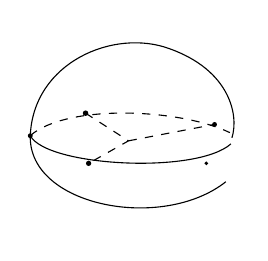
\begin{tikzpicture}[x=1.3cm,y=1.3cm]
\draw (-1,0) .. controls (-.97,.72) and (-.18,1.05) .. (.36,.85) .. controls (.95,.64) and (1.04,.20) .. (.97,-.02);
\draw (-1,0) .. controls (-1.02,-.69) and (.29,-.94) .. (.91,-.45);
\draw (-1,0) .. controls (-.84,-.30) and (.62,-.38) .. (.96,-.08);
\draw[dashed] (-1,0) .. controls (-.65,.31) and (.45,.27) .. (.95,.03);
\draw[dashed] (-.46,.22)--(-.04,-.05)--(-.43,-.27);
\draw[dashed] (-.04,-.05)--(.80,.11);
\fill (-1,0) circle (.024);\fill (-.46,.22) circle (.027);\fill (-.43,-.27) circle (.026);\fill (.80,.11) circle (.024);\fill (.72,-.27) circle (.019);
\end{tikzpicture}}
\deleted{Pour} tout $i\in I$, le cercle $\unsure{\Gamma|T}_{i\rho}\deleted{^{\unsure{\rho}}}$ admet deux pts \deleted{\unsure{marqués}} sur l'équateur, \deleted{\unsure{canoniquement marqués}}
\figure{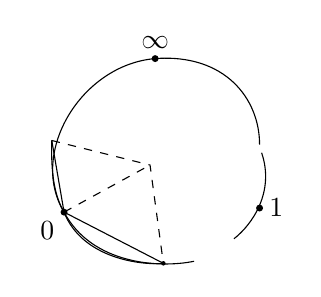
\begin{tikzpicture}[x=1.3cm,y=1.3cm]
\draw (-.89,-.50) .. controls (-1.24,.08) and (-.72,.94) .. (0,1) .. controls (.68,1.05) and (1.02,.61) .. (1.02,.16);
\draw (1.04,.08) .. controls (1.17,-.30) and (.95,-.62) .. (.77,-.76);
\draw (-.89,-.50) .. controls (-.62,-1.01) and (.04,-1.05) .. (.38,-.98);
\draw (-1.01,.20)--(-.89,-.50);
\draw (-1.01,.20) .. controls (-1.02,-.13) and (-.98,-.35) .. (-.89,-.50);
\draw (-.89,-.50)--(.08,-1);
\draw (-.89,-.50) .. controls (-.71,-.96) and (-.12,-1.02) .. (.08,-1);
\draw[dashed] (-1.01,.20)--(-.05,-.04)--(.08,-1);
\draw[dashed] (-.89,-.50)--(-.05,-.04);
\fill (0,1) circle (.034) node[above] {$\infty$};
\fill (1.02,-.46) circle (.034) node[right] {$1$};
\fill (-.89,-.50) circle (.034) node[below left] {$0$};
\fill (.08,-1) circle (.022);
\end{tikzpicture}}
\mspage{112}
\scanpage{114}
bijection canonique
\[
\Gamma_{i\rho}\cap\Sigma_{\mathbb R}\simeq I\setminus\{i\}
\]
en associant à $\forall x\in\Gamma_{i\rho}\cap\unsure{E_0|\Sigma_{\mathbb R}}$ l'élément de $I\setminus\{i\}$ le plus proche. Ces deux pts sont \unsure{diamétralmt|diamétralement} opposés sur $\Gamma_{i\rho}$, donc on trouve un isomorphisme canonique
\[
\Gamma_{i\rho}\simeq\deleted{\mathbb Z}\cdot\mathbb U\wedge_{\{\pm1\}}(I\setminus\{i\})
\]
ie. $\Gamma_{i\rho}$ est déduit du $\{\pm1\}$-torseur $I-\{i\}$ par l'inclusion
\[
\deleted{(\mathbb Z\times\unsure{\mu_2|\{\pm1\}})}\inserted{\{\pm1\}}\lhook\joinrel\longrightarrow\mathbb U.
\]

\deleted{la donnée de} La courbe $X_G$ du type $G$ s'obtient en prenant la normalisée
\[
\widetilde X_G=\coprod_{s\in\unsure{G|S}}\Sigma_{\widehat{\vec A}_s}
\]
par recollement à partir de l'involution $\sigma$ sur $\widehat{\vec A}=\coprod_{s\in S}\widehat{\vec A}_s$. On a pour $\forall x\in\widehat A$, au dessus de $s\in S$
\[
T_x\simeq\mathbb U\wedge_{\{\pm1\}}\{\widehat{\vec A}_s\setminus x\}
\qquad\text{si }x\in I\simeq\widehat{\vec A}^{\sigma}
\]
\inserted{(en identifiant les éléments de $I$ à leurs images dans $\widehat A$)}
\[
T_x\simeq\mathbb U\wedge_{\{\pm1\}}\bigwedge_{\widetilde x\in\widehat{\vec A}_x}
\bigl(\widehat{\vec A}_{\unsure{\sigma|o}(\widetilde x)}\setminus\{\widetilde x\}\bigr)
\qquad\text{si }x\in A
\]
\figure{\begin{tikzpicture}[x=1.05cm,y=1.05cm]
\coordinate (a) at (-2,-.65);\coordinate (b) at (-1.45,.12);\coordinate (c) at (-.65,.17);\coordinate (d) at (.55,.12);\coordinate (e) at (1.12,.80);\coordinate (f) at (1.48,.08);\coordinate (g) at (.85,-.50);\coordinate (h) at (1.22,1.40);
\draw (a)--(b)--(c)--(a);\draw (c)--(d)--(e)--(f)--(g)--(d);\draw (e)--(h);
\draw (h) .. controls (.75,1.85) and (1.00,2.22) .. (1.40,2.02) .. controls (1.90,1.85) and (1.57,1.56) .. (h);
\draw[->] (a)--(-2.12,.20);\draw[->] (b)--(-1.60,1.38);\draw[->] (f)--(2.18,.08);\draw[->] (g) .. controls (.91,-.88) and (.83,-1.03) .. (.80,-1.20);
\fill (a) circle (.024);\fill (b) circle (.030);\fill (c) circle (.023);\fill (d) circle (.030);\fill (h) circle (.035);
\end{tikzpicture}}
\uline{NB} Si $x$ est une boucle, on trouve $T_x\simeq\mathbb U$ iso. can.
\mspage{113}
\scanpage{115}
On a donc
\[
P_G=\prod_{x\in\widehat A}T_x
=\mathbb U^{\widehat A}\wedge_{\{\pm1\}^{\widehat A}}
\overbrace{\prod_{a\in\widehat A}\varepsilon_a}^{S\varepsilon_G}
\]
où pour $a\in\widehat A$, $\varepsilon_a$ est l'ens. à deux éléments défini par
\[
\begin{cases}
\varepsilon_a=\widehat{\vec A}_s-\{a\}&\text{si }a\in I\\
\varepsilon_a=\displaystyle\bigwedge_{\widetilde a\text{ sur }a}
\bigl(\widehat{\vec A}_{\unsure{\sigma|o}(\widetilde a)}\setminus\widetilde a\bigr)
&\text{si }a\in A=\widehat A\setminus I
\end{cases}
\]
et on trouve un \deleted{\unsure{applicati}} \inserted{morphisme} canonique
\[
\mu_{\vec A}^{\circ}\times SP_G\longrightarrow SPM_{G^\natural}
\qquad\text{où }\mu_{\vec A}^{\circ}=(]0,1[)^{\vec A}
\]
définissant
\[
\unsure{\Pi_1|\pi_1}(SP_G)=S\mathcal T_G=\mathbb Z^{\widehat A}
\longrightarrow\unsure{\Pi_1|\pi_1}(SPM_{G^\natural})=S\mathcal T_{G^\natural}
\]
et, mieux, un hom. de groupoïdes fondamentaux.

Mais \deleted{$\unsure{P_G}=\unsure{\prod_a\varepsilon_a|\{\prod_a\varepsilon_a\}}$} l'ensemble $\varepsilon_G$
(de cardinal $2^{\operatorname{card} A}$) est contenu dans $SP_G$
\[
S\varepsilon_G\subset SP_G
\]
d'où
\[
\mu_{\vec A}^{\circ}\times S\varepsilon_G\longrightarrow PM_{G^\natural}
\]
et comme $\mu_{\vec A}^{\circ}$ est simplement connexe, on en conclut
\[
S\varepsilon_G\longrightarrow\operatorname{Ob}(S\mathcal T_{G^\natural})
\]
(où $S\mathcal T_{?}$ désigne le groupoïde fondamental de $SP_{\unsure{?}}$)

\deleted{\unsure{J'entends dans ces}}
Désignons par $S_0\mathcal T_G$ le s/groupoïde de $S\mathcal T_G=\unsure{\Pi_1|\pi_1}(P_G\unsure{)}$
induit sur $S\varepsilon_G$, on a donc
\[
S_0\mathcal T_G\longrightarrow S\mathcal T_{G^\natural}.
\]
\mspage{114}
\scanpage{116}
Le groupoïde $S_0\mathcal T_G$ est engendré par les objets de
$S\varepsilon_G=\prod_{a\in\widehat A}\varepsilon_a$, et
\deleted{\unsure{des morphismes}} \inserted{pour \unsure{tt|$\forall$} système}
de signes
\deleted{$\varepsilon_a$}
\[
\alpha=(\alpha_a)\in\{\pm1\}^{\widehat A}
\]
et tout
\[
\unsure{\xi|\zeta}\in\varepsilon_G
\]
un morphisme
\[
u_{\alpha,\unsure{\xi|\zeta}}:\unsure{\xi|\zeta}\longrightarrow\alpha\unsure{\xi|\zeta}=\unsure{\xi|\zeta}'
\]
\margin{\inserted{défini par le chemin $u_{\alpha,\unsure{\xi|\zeta}}:[0,1]\longrightarrow P_G$}
\deleted{\unsure{donc}}
\deleted{(\unsure{défini} \illegible{2} de $SP$}
\deleted{$u_{\alpha,\unsure{\xi|\zeta}}(t)_a=$}
donné par
\[
u_{\alpha,\unsure{\xi|\zeta}}(t)_a=\begin{cases}
\unsure{\xi|\zeta}_a=\unsure{\xi|\zeta}'_a&\text{si }\alpha_a=+1\\
(\exp(\pi it))\unsure{\xi|\zeta}_a&\text{si }\alpha_a=-1
\end{cases}
\]}
avec les relations
\diagram{\begin{tikzcd}[column sep=large]
\unsure{\xi|\zeta}\arrow[r,"u_{\alpha,\unsure{\xi|\zeta}}"]\arrow[rr,bend right=30,"u_{\alpha\beta,\unsure{\xi|\zeta}}\,\unsure{n|u}(\alpha,\beta)"']
&\alpha.\unsure{\xi|\zeta}=\unsure{\xi|\zeta}'\arrow[r,"u_{\beta,\unsure{\xi|\zeta}'}"]
&\beta\unsure{\xi|\zeta}'=\deleted{\unsure{\alpha}}\beta\alpha\unsure{\xi|\zeta}=\unsure{\xi|\zeta}''
\end{tikzcd}}
où $\unsure{n|u}(\alpha,\beta)\in\mathbb Z^{\widehat A}$ donné par
\deleted{$\{\unsure{n|u}(\alpha,\beta)_a=0$ \unsure{sauf si}
\inserted{si $\alpha_a=1$ ou $\unsure{\beta_a}$}}
\[
\unsure{n|u}(\alpha,\beta)_a=\begin{cases}
0&\text{si }\alpha_a=1\text{ ou }\beta_a=1\\
1&\text{sinon (i.e }\alpha_a=\beta_a=-1\text{)}
\end{cases}
\]

On \deleted{\unsure{peut}} a tenu compte, pour écrire \unsure{ces} relations,
de la $\mathbb Z^{\widehat A}$-structure du groupoïde $S_0\mathcal T_G$.
Si on veut pas l'utiliser, on introduira, pour $a\in\widehat A$, $\unsure{\xi|\zeta}\in\varepsilon_G$
\[
u_{a,\unsure{\xi|\zeta}}:\unsure{\xi|\zeta}\longrightarrow\sigma_a\unsure{\xi|\zeta}
\]
\margin{NB $\sigma_a$ désigne l'involution de $S\varepsilon_G$ associée à $a\in\widehat A$}
et les relations deviennent
\[
(1)\qquad
\diagram{\begin{tikzcd}[column sep=large,row sep=large]
\unsure{\xi|\zeta}\arrow[r,"u_{a,\unsure{\xi|\zeta}}"]\arrow[d,"u_{b,\unsure{\xi|\zeta}}"']&\sigma_a\unsure{\xi|\zeta}\arrow[d,"u_{b,\sigma_a\unsure{\xi|\zeta}}"]\\
\sigma_b\unsure{\xi|\zeta}\arrow[r,"u_{a,\sigma_b\unsure{\xi|\zeta}}"']&\sigma_{ab}
\end{tikzcd}}
\]
commutatif
$(\forall(\unsure{\xi|\zeta},a,b)\in S\varepsilon_G\times\widehat A\times\widehat A)$
il suffit de le \unsure{poser|prouver} pour $a\ne b$
\mspage{115}
\scanpage{117}
(2) \deleted{\unsure{Posons} $u_a$}
\inserted{Soit $v^a_{\unsure{\xi|\zeta}}$ le composé}
\diagram{\begin{tikzcd}[column sep=large]
\unsure{\xi|\zeta} \arrow[r,"u_{a,\unsure{\xi|\zeta}}"] & a\unsure{\xi|\zeta} \arrow[r,"u_{a,a\unsure{\xi|\zeta}}"] & a^2\unsure{\xi|\zeta}=\unsure{\xi|\zeta}
\end{tikzcd}}
alors les $v^a_{\unsure{\xi|\zeta}}$ commutent ($\unsure{\xi|\zeta}$ fixé, $a\in\widehat{A}$ \unsure{variab.}).

\margin{\uline{\unsure{NB}}}
Le groupoïde libre sur les \deleted{\unsure{objets de}} \inserted{$\varepsilon_G$ comme} ens. d'objets, et avec les générateurs $u_{a,\unsure{\xi|\zeta}}$ et les relations (1) (2), \deleted{est} s'identifie bien à $S_0\mathcal{T}_G$ (à isom. can. près).

\unsure{Prenant} $\mathcal{T}_G$, au \deleted{\unsure{point}} lieu de $S_0\mathcal{T}_G$, on trouve une construction \deleted{\unsure{analogue}} \inserted{\unsure{parallèle}} \deleted{en} termes de \deleted{$\varepsilon_{G,A}$ \unsure{(quotient de} $\varepsilon$}
\[
\varepsilon_G=\prod_{a\in A}\varepsilon_a\subset P_G=\prod_{a\in A}T_a
\]
qui est l'ens des objets d'un groupoïde \inserted{\unsure{conn.}} ${}_0\mathcal{T}_G$, \deleted{décrit} de groupe fondamental abélien $\mathbb{Z}^A$, décrit mutatis mutandis, comme $S_0\mathcal{T}_G$ à partir des $\unsure{S\varepsilon_G|S_{\varepsilon_G}}$. On a alors
\diagram{\begin{tikzcd}[column sep=large,row sep=large]
S_0\mathcal{T}_G \arrow[r] \arrow[d] & S\mathcal{T}_{G^{\unsure{\natural|\sharp}}} \arrow[d] \\
{}_0\mathcal{T}_G \arrow[r] & \mathcal{T}_{G^{\unsure{\natural|\sharp}}}
\end{tikzcd}}
\mspage{116}
\scanpage{118}
\uline{Dimension modulaire 1} Tous les sommets de $G$, sauf un seul $s_0$, sont de genre $0$ et d'ordre $3$, tandis que $s_0$ est soit de genre $0$, ordre $4$, soit de genre $1$, ordre $1$.

\figure{\begin{tikzpicture}[scale=.8]
\fill (0,0) circle (2pt);
\draw (0,0)--(-.8,.38) (0,0)--(-.4,.72) (0,0)--(.37,.72) (0,0)--(.95,.63);
\draw[densely dotted] (-1.55,.48)--(-.92,.55) (-1.05,.92)--(-.5,.96) (-.21,.96)--(.36,.92) (.82,.85)--(1.33,.91);
\node[below] at (0,0) {$s_0$};
\draw[densely dotted] (3.8,.3)--(4.4,.3);
\draw (4.7,.32)--(6.2,.4);
\fill (6.2,.4) circle (2pt);
\node[below] at (6.2,.4) {$1$};\node[right] at (6.45,.25) {$s_0$};
\end{tikzpicture}}

Traitons d'abord le premier cas. Soit $I=\widehat{\vec A}_{s_0}$, ens. de cardinal $4$. On a un iso canonique
\[
M_G\simeq M_{0,I}\qquad
(\simeq\overbrace{\mathbb{P}^1_{\mathbb{C}}\setminus\{0,1,\infty\}}^{\mathbb{U}_{0,3}},
\]
\margin{isomorphisme qui dépend d'une \unsure{ordination|ordonnation} des éléments de $I$}
\[
\deleted{\unsure{SP_G}\simeq}
\]
La donnée d'une courbe $X$ de type $G$ équivaut à celle d'une \deleted{\unsure{sphère}} droite projective \inserted{$Y$} $I$-marquée.

On a
\[
\begin{aligned}
M_{0,I}&=\deleted{M_{0,4}\wedge}\operatorname{Rep}(I)\wedge_{\unsure{\mathfrak{S}_4|\mathfrak{G}_4}}M^!_{0,4}\\
&=\operatorname{Rep}(I)\wedge_{\unsure{\mathfrak{S}_4|\mathfrak{G}_4}}\mathbb{U}_{0,3}
\end{aligned}
\]
\margin{NB $\operatorname{Rep}(I)=\operatorname{Bij}(I_4,I)$ avec $I_4=\mathbb{N}\cap[1,4]$}
où $\unsure{\mathfrak{S}_4|\mathfrak{G}_4}$ opère sur $\mathbb{U}_{0,3}$ par l'intermédiaire de l'action du groupe $\unsure{\mathfrak{S}_3|\mathfrak{G}_3}$ et de l'homomorphisme
\diagram{\begin{tikzcd}
\unsure{\mathfrak{S}_4|\mathfrak{G}_4}\arrow[r] & \unsure{\mathfrak{S}_3|\mathfrak{G}_3}
\end{tikzcd}}
où $\unsure{\mathfrak{S}_3|\mathfrak{G}_3}$ est identifié au \deleted{\unsure{l'ensemble}} \inserted{groupe} des permutations de l'ens des partitions de type $2,2$ de l'ens à $4$ éléments $[1,4]\cap\mathbb{N}=I_4$, ces partitions étant numérotées de $1$ à $3$, la partition \uline{$P_i$} ($1\leq i\leq3$) étant \inserted{formée de} $\{i,4\}$ et de son complémentaire \deleted{$\unsure{I_4}$} $I_3\setminus\{i\}$ dans $I_4$. On aura, si $T_i$ ($i\in I$) sont les fibrés tangents unitaires de $Y$ aux pts de $I=\widehat{\vec A}_{s_0}$, pour \deleted{$\unsure{P}$} $a\in A$ :
\mspage{117}
\scanpage{119}
\margin{Si $s_0$ n'est pas un sommet de $a$}
\[
T_a=\mathbb{U}\wedge_{\{\pm1\}}\varepsilon_a\qquad\text{pour}\qquad
\varepsilon_a=\begin{cases}
\widehat{\vec{A}}_{\unsure{o|\sigma}(x)}\setminus x&\text{si }x\in I_s\quad\deleted{\unsure{\widehat{A}}}\\
\displaystyle\bigwedge_{\widetilde{x}\in\widehat{\vec{A}}_x}(\widehat{\vec{A}}_{o(\widetilde{x})}\setminus\{\widetilde{x}\})&\text{si }x\in A
\end{cases}
\]
\deleted{\unsure{Si $s_0$ est}} Si $s_0$ est un sommet de $a$, on est dans l'un des \inserted{trois} cas ci-dessous, \unsure{suiv.} que $a\in I$, \inserted{\unsure{que $a$}} $\Bigl\{$ \deleted{\unsure{est une arête liée}} \inserted{\unsure{ou une arête non pas bouclée|ou est une arête non bouclée}}, est une boucle, \deleted{\illegible{1}} \deleted{\unsure{liée}} Mais dans tous les cas on a

\figure{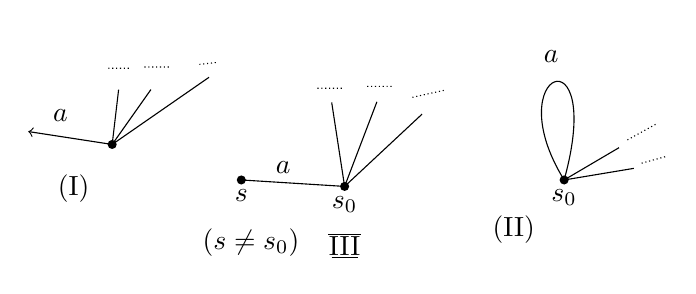
\begin{tikzpicture}[scale=.82]
\fill (0,0) circle (2pt);
\draw[->] (0,0)--(-1.3,.2);\node[above] at (-.8,.2) {$a$};
\draw (0,0)--(.1,.85) (0,0)--(.6,.85) (0,0)--(1.5,1.04);
\draw[densely dotted] (-.06,1.18)--(.26,1.18) (.5,1.2)--(.9,1.2) (1.35,1.24)--(1.62,1.27);
\node[below left] at (-.2,-.32) {$(\mathrm{I})$};
\fill (2,-.55) circle (2pt);\node[below] at (2,-.55) {$s$};
\fill (3.6,-.65) circle (2pt);\node[below] at (3.6,-.65) {$s_0$};
\draw (2,-.55)--(3.6,-.65);\node[above] at (2.65,-.6) {$a$};
\draw (3.6,-.65)--(3.4,.65) (3.6,-.65)--(4.1,.66) (3.6,-.65)--(4.8,.47);
\draw[densely dotted] (3.18,.87)--(3.59,.87) (3.95,.9)--(4.35,.9) (4.65,.73)--(5.15,.84);
\node[below] at (2.15,-1.15) {$(s\ne s_0)$};\node at (3.6,-1.57) {$\mathrm{III}$};\draw (3.35,-1.4)--(3.85,-1.4) (3.4,-1.75)--(3.8,-1.75);
\fill (7,-.55) circle (2pt);\node[below] at (7,-.55) {$s_0$};
\draw (7,-.55)..controls(5.95,1.15)and(7.65,1.8)..(7,-.55);
\node[above] at (6.8,1.12) {$a$};
\draw (7,-.55)--(7.85,-.05) (7,-.55)--(8.08,-.37);
\draw[densely dotted] (7.98,.07)--(8.45,.33) (8.2,-.29)--(8.6,-.18);
\node[below left] at (6.7,-.95) {$(\mathrm{II})$};
\end{tikzpicture}}
\[
T_a=\bigwedge_{\widetilde{a}\in\unsure{A}}T_{\widetilde{a}}\quad
\begin{cases}
T_i&\begin{gathered}\text{dans cas (I) où }i\in J=\widehat{\vec{A}}_{s_0}\text{ est l'élément}\\\text{qui correspond à l'unique }\vec a\text{ sur }a\end{gathered}\\[1.3em]
\displaystyle\bigwedge_{\substack{i\in J\\\text{au dessus}\\\text{de }a}}T_i&\text{dans cas (II)}\\[1.3em]
T_i\wedge_{\{\pm1\}}(\widehat{\vec{A}}_s-\{\vec a\})&\begin{gathered}\text{dans le cas (III),}\\\text{où }\vec a\text{ désigne}\\\text{l'arc d'origine }s\ne s_0\text{ porté par }a\end{gathered}
\end{cases}
\]

On trouve donc
\[
SP_X=\prod_{a\in\widehat{A}}T_a
\]
et avec l'explicitation des $T_a$ par les formules précédentes, on voit que chaque $T_i$ ($i\in J$) intervient dans le produit une fois et une seule, mais sous forme tordue si $i\in J=\widehat{\vec{A}}_{s_0}$ correspond à \unsure{une|un} \unsure{arc|arête} qui est lié et pas une boucle.

Soit donc $\widehat{A}_1\subset\widehat{A}$ l'ens des arêtes de $G$ qui \deleted{\unsure{partent}} n'ont pas \deleted{\unsure{d'autre}} $s_0$ comme extrémité, \deleted{\unsure{liées de par les bords}} \deleted{\unsure{ou que de la contraction}\ \illegible{5}}
\mspage{118}
\scanpage{120}
\deleted{Posons, pour $a\in A_1$,}
\[
\deleted{\varepsilon_a=\left\{\begin{gathered}\text{ce qui est défini pg. précédente, \unsure{si $s_0$ pas}}\\\text{un sommet de }a\end{gathered}\right.}
\]
et $J_1$ l'ens des éléments de $J=\widehat{\vec A}_{s_0}$ qui sont \deleted{\unsure{liés}} des arcs liés pas boucles, $J_2=J\setminus J_1$. On aura alors, posant
\[
\varepsilon_{\widehat{A}_1}=\prod_{a\in\widehat{A}_1}\varepsilon_a,
\]
\[
SP_X=\underbrace{\left(\mathbb{U}^{A_1}\wedge_{\{\pm1\}^{A_1}}\varepsilon_{A_1}\right)}_{T_{A_1}}\times T_J^Y,
\]
où
\[
T_J^Y=\prod_{a\in\widehat{A}\unsure{\setminus}\widehat{A}_1}T_a
\]
\margin{(produit d'au moins deux \deleted{\unsure{fbts}} au plus quatre facteurs}
\margin{$A\setminus A_1={}$ens des arêtes incidentes à $s_0$}

où $T_J^Y$ est \inserted{\unsure{ainsi}} défini directement en termes de $Y$ et des ens. \inserted{à deux éléments} $\widehat{\vec A}_s\setminus\{\vec a\}$ relatifs aux \deleted{sommets} \inserted{arcs $a\in\widehat{\vec A}_{s_0}=J$} qui sont liés et pas des boucles, $s$ désignant l'extrémité \deleted{\unsure{$s$ distinct de $s_0$ et adjacent à $s_0$}} dudit arc --- en \unsure{supposant} de plus \unsure{connu|connus} le groupage \unsure{d'|de}\inserted{certains} éléments de $J$ en \inserted{une ou deux} paires (disjointes dans le cas de deux paires), quand il y a une ou deux boucles de $G$ en $s_0$. De façon précise, par la structure de $G$ dont $J$ provient, on a
\[
J=J_{\mathrm{I}}\amalg J_{\mathrm{II}}\amalg J_{\mathrm{III}}
\]
où $J_{\mathrm{II}}$ est muni d'une involution sans pts fixes $\unsure{\sigma_{\mathrm{II}}}$.
et où $J_{\mathrm{III}}$ est muni d'un rev. de degré $2$
\diagram{\begin{tikzcd}\widetilde{J}_{\mathrm{III}}\arrow[r]&J_{\mathrm{III}}\end{tikzcd}}
On aura alors, \unsure{en termes de} cette structure de $J$
\[
T_J^Y=T_{J_{\mathrm{I}}}^Y\unsure{*|\times}T_{J_{\mathrm{II}}}^Y\unsure{*|\times}T_{J_{\mathrm{III}}}^Y
\]
\mspage{119}
\scanpage{121}
avec
\[
T_{J_{\mathrm{I}}}^Y=\prod_{i\in J_{\mathrm{I}}}T_i
\]
\[
T_{J_{\mathrm{II}}}^{\unsure{1|Y}}=
\underbrace{\prod_{\alpha\in J_{\mathrm{II}}/\sigma}}_{\substack{0,1\text{ ou }2\\\text{facteurs}}}
\underbrace{\bigwedge_{\substack{i\in J_{\mathrm{II}}\\\text{sur }\alpha}}T_i}_{2\text{ facteurs}}
\]
\[
T_{J_{\mathrm{III}}}^Y=\prod_{i\in J_{\mathrm{III}}}T_i\wedge_{\{\pm1\}}\widetilde{J}_{\mathrm{III},i}
\]
Il est clair que pour $Y$ variable, les $T_{J_{\mathrm{I}}}^Y$, $\unsure{J_{J_{\mathrm{II}}}^Y|T_{J_{\mathrm{II}}}^Y}$, $T_{J_{\mathrm{III}}}^Y$ forment des \deleted{fibrés} \inserted{$\mathbb{U}$-torseurs} sur $M_{0,I}$, soient $T_{\mathrm{I}}$, $T_{\mathrm{II}}$, $T_{\mathrm{III}}$, dont le produit fibré sera noté $T_{A_2}$ si
\[
A_2=A\setminus A_1\simeq J_{\mathrm{I}}\amalg(J_{\mathrm{II}}/\sigma)\amalg J_{\mathrm{III}}.
\]
On \unsure{écrit|aura} donc
\[
SP_G\simeq
\underbrace{T_{\widehat{A}_1}}_{\mathbb{U}^{\widehat{A}_1}\text{-torseur}}
\times
\underbrace{T_{\widehat{A}_2}}_{\substack{\mathbb{U}^{A_2}\text{ torseur}\\\text{sur }M_{0,\unsure{J|I}}}}
\]
Nous allons maintenant décrire un avatar du groupoïde fondamental de $SP_G$, i.e. de $S\mathcal{T}_G$, par le choix de ``pts bases'' bien choisis. On va s'intéresser aux $Y$ qui correspondent aux $\unsure{5|6}$ pts de $M_{0,I}$ qui sont des pts de ramification pour l'action du groupe quotient $\unsure{\mathfrak{S}_{J'}|\mathfrak{G}_{J'}}$ de $\unsure{\mathfrak{S}_J|\mathfrak{G}_J}$ (où $J'\in\deleted{\unsure{\mathcal{E}|\widehat{A}}}(3\text{-Ens})$ est l'ens des trois partitions de
\mspage{120}
\scanpage{122}
type $2,2$ de $J$. Ces points correspondent aux droites projectives $J$-marquées qui ont des automorphismes \deleted{non triviaux} \inserted{d'ordre $>4$}, il y en a de deux sortes :
\margin{ils sont \unsure{toujours} d'ordre multiple de $4$}

a) Pour \unsure{$\forall$|tt} structure ``carré'' sur $J$, correspondant à une partition de type $(2,2)$, on a un plongement canonique de $\unsure{Y|J}$ dans une \unsure{droite|quadrique} projective, de façon que les \deleted{\unsure{groupe des}} \inserted{$8$ autom.} \deleted{\unsure{autres}} du carré soient induits par des \unsure{autom.} projectifs. Si $Q$ est une structure carré sur $J$, on désignera par $Y_Q$ la droite projective correspondante. \deleted{\unsure{Il}}

\figure{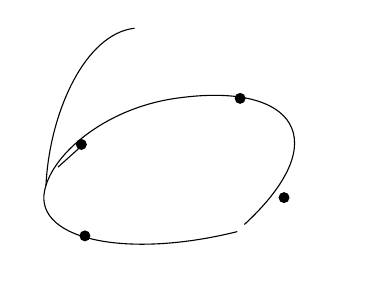
\begin{tikzpicture}[scale=.9]
\draw (0,0)..controls(-.25,-.75)and(1.1,-1.05)..(2.7,-.65);
\draw (2.8,-.55)..controls(4.1,.65)and(3.5,1.45)..(1.9,1.24)..controls(.9,1.12)and(.15,.5)..(0,0);
\fill (.5,.58) circle (2.2pt);\fill (2.74,1.23) circle (2.2pt);\fill (3.36,-.17) circle (2.2pt);\fill (.55,-.71) circle (2.2pt);
\draw (0,0)..controls(.05,1.03)and(.55,2.14)..(1.25,2.22);
\draw (.17,.26)--(.56,.61);
\end{tikzpicture}}

Le groupe des rotations du carré opère de façon simplement transitive sur l'ens $J$, de sorte que les $T_i$ s'identifient entre eux. Si $\omega_Q$ est l'ens des deux orientations du carré, \deleted{qui est \unsure{associé can.} $\unsure{1-1}$ \unsure{avec} l'ens $\omega_J$ des deux orientations de l'ens $J$,} on a un isom canonique
\[
T_i=\mathbb{U}\times_{\{\pm1\}}\omega_Q
\]
en choisissant comme origine \inserted{en $i$ associée à une orientation} la direction \uline{tangente}
\mspage{121}
\scanpage{123}
à l'équateur, dans le sens de cette orientation.

On aura alors
\[
\deleted{T_{\widehat A_2}^{\unsure{Y}}=\mathbb U^A}
\]
\[
T_{J_{\mathrm I}}^Y=\mathbb U^{J_{\mathrm I}}\mathop{\wedge}_{\{\pm1\}}\omega_Q
\]
\margin{NB $\{\pm1\}$ s'envoie diagonalement dans $\mathbb U^{J_1}$}
\[
T_{J_{\mathrm {II}}}^Y\simeq\mathbb U^{J_2}
\]
\margin{car $\displaystyle\bigwedge_{\substack{i\in J_{\mathrm{II}}\\\text{sur }\alpha}}T_i\simeq\mathbb U$, puisque les $T_i$ sont isomorphes can. à $\mathbb U\mathop{\wedge}_{\pm1}\omega_Q$, donc le produit contracté de deux d'entre eux est $\mathbb U$}
\[
T_{J_{\mathrm{III}}}^Y\simeq
\prod_{i\in J_{\unsure{\mathrm{II}|\mathrm{III}}}}
\mathbb U\mathop{\wedge}_{\{\pm1\}}
\underbrace{(\omega_Q\wedge\widetilde J_{\mathrm{III},i})}_{\varepsilon_i}
\]

Donc, si $J_{\mathrm I}\ne\varnothing$, on introduit l'ensemble
\[
\unsure{\varepsilon|\mathcal E}_{G,Q}=\varepsilon_{G,Y_Q}
=\underbrace{\varepsilon_{\widehat A_1}}_{\displaystyle\prod_{a\in\widehat A_1}\varepsilon_a}
\times\omega_Q\times
\underbrace{\varepsilon_{J_{\mathrm{III}}}}_{\displaystyle\prod_{i\in J_{\mathrm{III}}}\omega_Q\wedge\widetilde J_{\mathrm{III},i}}
\]
qui est un torseur sous
\[
\gamma_{\unsure{G_s|G}}=\{\pm1\}^{\widehat A_1}\times\{\pm1\}\times\{\pm1\}^{J_{\mathrm{III}}}
\]
groupe qui s'envoie dans $\mathbb U^{\widehat A}$
\diagram{\begin{tikzcd}[column sep=large,row sep=small]
\gamma_G\arrow[r]\arrow[dr,bend right=18]&
\mathbb U^{\widehat A}\unsure{\simeq|=}\mathbb U^{\widehat A_1}\times
\mathbb U^{J_{\mathrm I}}\times
\mathbb U^{J_{\mathrm{II}}/\sigma}\times\mathbb U^{J_{\mathrm{III}}}\\
&\mathbb U^{\widehat A_1}\times\overset{\unsure{\smile|\vee}}{\mathbb U^{J_1}}\times\mathbb U^{J_{\mathrm{III}}}
\end{tikzcd}}
\deleted{\unsure{en f}}

en factorisant par le produit triple, et en

\mspage{122}
\scanpage{124}
prenant le produit cartésien de
\diagram{\begin{tikzcd}
\{\pm1\}^{A_1}\arrow[r,hook]&\mathbb U^{A_1}
\end{tikzcd}}
\margin{hom. évident déduit de $\{\pm1\}\hookrightarrow\mathbb U$}
\diagram{\begin{tikzcd}
\{\pm1\}\arrow[r,hook]\arrow[dr,"{\text{diag}}"']&\mathbb U^{J_{\mathrm I}}\\
&\{\pm1\}^{J_{\mathrm I}}\arrow[u,hook,"{\text{incl. can}}"']
\end{tikzcd}}
\diagram{\begin{tikzcd}
\{\pm1\}^{J_{\mathrm{III}}}\arrow[r,hook]&\mathbb U^{J_{\mathrm{III}}}
\end{tikzcd}}
\margin{hom. évident.}

Ceci posé, \unsure{enf}, on aura
\[
SP_G^Y\simeq\mathbb U^{\widehat A}\mathop{\wedge}_{\gamma_G}
\underbrace{\varepsilon_{G,Q}}_{\gamma_G\text{-tors.}}
\]

Dans le cas où $J_{\mathrm I}=\varnothing$, on \inserted{peut} poser si on préfère
\[
\varepsilon_{G,Q}=\varepsilon_{G,Y_Q}=\varepsilon_{\widehat A_1}\times\varepsilon_{J_{\mathrm{III}}}
\]
faisant l'économie du facteur $\omega_Q$, \unsure{définissons}
\[
\gamma_G=\{\pm1\}^{\widehat A_1}\times\{\pm1\}^{J_{\mathrm{III}}}
=\{\pm1\}^{\widehat A_1\amalg J_{\mathrm{III}}}
\]
et on \unsure{conservera|conserve} l'expression ci-dessus pour $SP_G^Y$.

Considérons donc
\[
S_0\mathcal T_G^{Y_Q}=S_0\mathcal T_G^Q
\]
\margin{sous-groupoïde plein de $\unsure{\Pi_1|\mathbb{\Pi}_1}(SP_G^Y)$ basé en les éléments de $\varepsilon_{G,Q}$}

Il faudra expliciter ce groupoïde \deleted{fondamental} \inserted{basé sur $\varepsilon_{G,\unsure{Q}}$} par flèches \unsure{génératrices|générateurs} et relations -- j'y reviendrai.

\mspage{123}
\scanpage{125}
Je vais d'abord passer au deuxième cas de \deleted{\unsure{tels|la}} $Y$ exceptionnels :

Cas où il existe $i_0\in J$ tel que les autom de $(Y,J)$ fixant $i$ forment un groupe d'ordre $3$

\deleted{Ces $Y$ correspondent \unsure{biunivoquement} aux structures la donnée d'un $i_0\in J$ et d'un \unsure{triangulaire} $\unsure{i_0}$ ordre circulaire}

\figure{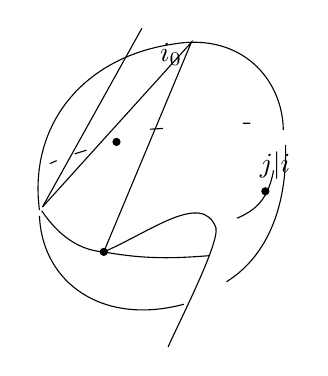
\begin{tikzpicture}[scale=.95]
\draw (0,.9) .. controls (-.15,2.05) and (.6,2.95) .. (1.8,3.12) .. controls (2.7,3.27) and (3.25,2.65) .. (3.26,1.97);
\draw (0,.82) .. controls (.04,-.08) and (.85,-.65) .. (1.93,-.36);
\draw (2.5,-.06) .. controls (3.09,.31) and (3.31,1.02) .. (3.29,1.77);
\draw (.04,.94)--(2.03,3.14)--(.86,.34);
\draw (.04,.94)--(1.37,3.33);
\draw (.03,.89) .. controls (.26,.55) and (.54,.36) .. (.86,.34) .. controls (1.45,.23) and (1.88,.26) .. (2.28,.29);
\draw (.86,.34) .. controls (1.47,.6) and (2.18,1.16) .. (2.36,.66) .. controls (2.4,.44) and (1.88,-.57) .. (1.72,-.93);
\draw (.14,1.52)--(.23,1.56) (.47,1.65)--(.63,1.7) (1.48,1.98)--(1.65,1.99) (2.72,2.06)--(2.82,2.06);
\fill (1.03,1.81) circle (.055);
\fill (.86,.34) circle (.055);
\fill (3.02,1.15) circle (.055);
\draw (2.64,.79) .. controls (2.9,.9) and (3.06,1.05) .. (3.13,1.43);
\node at (1.76,2.98) {$i_0$};
\node at (3.15,1.5) {$\unsure{j|i}$};
\end{tikzpicture}}

(Il revient au $=$ de dire que le groupe autom de $(Y,J)$ est le sous-groupe \inserted{alterné} $\unsure{\mathfrak S|\mathfrak G}_J^+$ de $\unsure{\mathfrak S|\mathfrak G}_J$, ou encore que la configuration est la configuration de la sphère circonscrite au tétraèdre\inserted{\unsure{C. analytique orienté})}. Les $2$ possibilités correspondent aux deux orientations de $J$, soit $\omega_J$ l'une de ces orientations. Le groupe d'isotropie d'un point $i$ est isomorphe au groupe des permutations circulaires sur l'ens des trois autres points qui \unsure{forment|forme} un torseur sous $\inserted{\mu_3=\mu_3(\mathbb C)\simeq}\mathbb Z/3\mathbb Z$, soit $\eta_i$ $(i\in I)$. On a

\figure{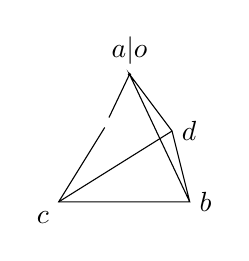
\begin{tikzpicture}[scale=.9]
\coordinate (a) at (1,1.8);
\coordinate (b) at (1.85,0);
\coordinate (c) at (0,0);
\coordinate (d) at (1.6,1.0);
\draw (a)--(.71,1.19);
\draw (.65,1.05)--(c)--(b)--(a)--(d)--(b);
\draw (c)--(d);
\fill (a) circle(.025);
\node[above] at (a) {$\unsure{a|o}$};
\node[right] at (b) {$b$};
\node[below left] at (c) {$c$};
\node[right] at (d) {$d$};
\end{tikzpicture}}

alors
\[
T_i\simeq\mathbb U\mathop{\times}_{\unsure{\deleted{\mathbb Z}|2}\mu_3}\eta_i
\]
où $\mu_3\hookrightarrow\mathbb U$ est l'inclusion canonique.

On

\mspage{124}
\scanpage{126}
\unsure{Graphes} MD

\margin{(6 p)}

\mspage{125}
\scanpage{127}
\figure{
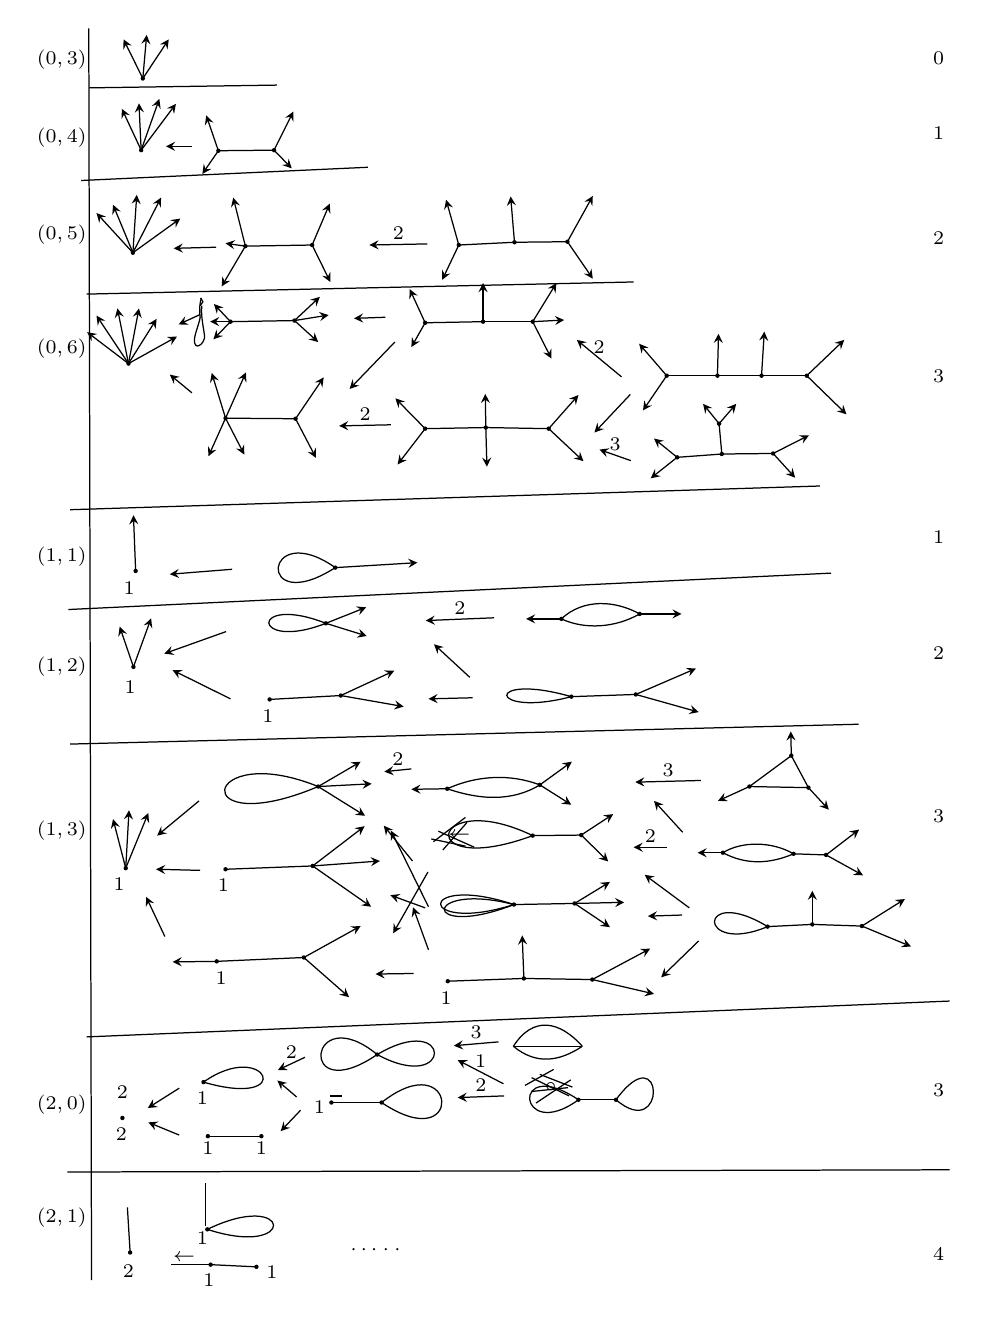
\begin{tikzpicture}[x=0.007cm,y=-0.007cm,line width=0.45pt,>=stealth,font=\scriptsize]
\draw (94,20) -- (99,2290);
\draw (95,128) -- (435,123);
\draw (80,296) -- (600,272);
\draw (90,502) -- (1082,480);
\draw (60,893) -- (1420,850);
\draw (57,1074) -- (1440,1008);
\draw (60,1318) -- (1490,1282);
\draw (90,1849) -- (1655,1784);
\draw (55,2094) -- (1655,2090);
\node at (45,77) {$(0,3)$};
\node at (1635,75) {$0$};
\draw[->] (192,111) -- (157,40);
\draw[->] (192,111) -- (199,32);
\draw[->] (192,111) -- (239,40);
\fill (192,111) circle[radius=4];
\node at (45,219) {$(0,4)$};
\node at (1635,211) {$1$};
\draw[->] (189,241) -- (154,166);
\draw[->] (189,241) -- (185,156);
\draw[->] (189,241) -- (222,148);
\draw[->] (189,241) -- (252,157);
\fill (189,241) circle[radius=4];
\draw (329,242) -- (430,241);
\draw[->] (329,242) -- (307,178);
\draw[->] (329,242) -- (300,284);
\draw[->] (430,241) -- (465,171);
\draw[->] (430,241) -- (462,274);
\fill (329,242) circle[radius=4];
\fill (430,241) circle[radius=4];
\draw[->] (282,234) -- (234,234);
\node at (45,394) {$(0,5)$};
\node at (1635,400) {$2$};
\draw[->] (174,427) -- (108,355);
\draw[->] (174,427) -- (138,340);
\draw[->] (174,427) -- (181,322);
\draw[->] (174,427) -- (225,327);
\draw[->] (174,427) -- (260,365);
\fill (174,427) circle[radius=4];
\draw (378,415) -- (499,413);
\draw[->] (378,415) -- (356,327);
\draw[->] (378,415) -- (342,410);
\draw[->] (378,415) -- (335,488);
\draw[->] (499,413) -- (531,338);
\draw[->] (499,413) -- (532,480);
\fill (378,415) circle[radius=4];
\fill (499,413) circle[radius=4];
\draw (765,413) -- (866,408);
\draw (866,408) -- (962,407);
\draw[->] (765,413) -- (742,331);
\draw[->] (765,413) -- (735,476);
\draw[->] (866,408) -- (859,325);
\draw[->] (962,407) -- (1008,324);
\draw[->] (962,407) -- (1008,474);
\fill (765,413) circle[radius=4];
\fill (866,408) circle[radius=4];
\fill (962,407) circle[radius=4];
\draw[->] (325,417) -- (248,419);
\draw[->] (708,411) -- (603,413);
\node at (655.5,392.0) {$2$};
\node at (45,601) {$(0,6)$};
\node at (1635,651) {$3$};
\draw[->] (166,628) -- (91,571);
\draw[->] (166,628) -- (108,541);
\draw[->] (166,628) -- (146,528);
\draw[->] (166,628) -- (185,528);
\draw[->] (166,628) -- (217,547);
\draw[->] (166,628) -- (254,579);
\fill (166,628) circle[radius=4];
\draw (351,552) -- (467,550);
\draw[->] (351,552) -- (321,520);
\draw[->] (351,552) -- (314,552);
\draw[->] (351,552) -- (320,584);
\draw[->] (467,550) -- (513,507);
\draw[->] (467,550) -- (529,540);
\draw[->] (467,550) -- (510,589);
\fill (351,552) circle[radius=4];
\fill (467,550) circle[radius=4];
\draw (704,554) -- (809,552);
\draw (809,552) -- (899,552);
\draw[->] (704,554) -- (676,493);
\draw[->] (704,554) -- (679,598);
\draw[->] (809,552) -- (809,482);
\draw[->] (899,552) -- (942,482);
\draw[->] (899,552) -- (956,549);
\draw[->] (899,552) -- (933,619);
\fill (704,554) circle[radius=4];
\fill (809,552) circle[radius=4];
\fill (899,552) circle[radius=4];
\draw (1142,650) -- (1234,650);
\draw (1234,650) -- (1314,650);
\draw (1314,650) -- (1396,650);
\draw[->] (1142,650) -- (1092,592);
\draw[->] (1142,650) -- (1099,713);
\draw[->] (1234,650) -- (1236,574);
\draw[->] (1314,650) -- (1319,570);
\draw[->] (1396,650) -- (1464,585);
\draw[->] (1396,650) -- (1468,720);
\fill (1142,650) circle[radius=4];
\fill (1234,650) circle[radius=4];
\fill (1314,650) circle[radius=4];
\fill (1396,650) circle[radius=4];
\draw (342,727) -- (469,728);
\draw[->] (342,727) -- (317,645);
\draw[->] (342,727) -- (379,644);
\draw[->] (342,727) -- (311,796);
\draw[->] (342,727) -- (376,793);
\draw[->] (469,728) -- (520,653);
\draw[->] (469,728) -- (506,799);
\fill (342,727) circle[radius=4];
\fill (469,728) circle[radius=4];
\draw (704,746) -- (814,744);
\draw (814,744) -- (928,746);
\draw[->] (704,746) -- (650,691);
\draw[->] (704,746) -- (654,811);
\draw[->] (814,744) -- (813,683);
\draw[->] (814,744) -- (816,815);
\draw[->] (928,746) -- (982,685);
\draw[->] (928,746) -- (991,805);
\fill (704,746) circle[radius=4];
\fill (814,744) circle[radius=4];
\fill (928,746) circle[radius=4];
\draw (1161,798) -- (1242,792);
\draw (1242,792) -- (1335,791);
\draw (1242,792) -- (1237,737);
\draw[->] (1161,798) -- (1119,764);
\draw[->] (1161,798) -- (1113,836);
\draw[->] (1335,791) -- (1400,758);
\draw[->] (1335,791) -- (1375,835);
\draw[->] (1237,737) -- (1208,701);
\draw[->] (1237,737) -- (1268,701);
\fill (1161,798) circle[radius=4];
\fill (1242,792) circle[radius=4];
\fill (1335,791) circle[radius=4];
\fill (1237,737) circle[radius=4];
\draw[->] (281,681) -- (241,648);
\draw[->] (632,544) -- (575,546);
\draw[->] (649,589) -- (567,674);
\draw[->] (642,739) -- (548,741);
\node at (595.0,720.0) {$2$};
\draw[->] (1060,652) -- (979,585);
\node at (1019.5,598.5) {$2$};
\draw[->] (1076,684) -- (1011,753);
\draw[->] (1077,804) -- (1020,784);
\node at (1048.5,774.0) {$3$};
\draw[->] (296,539) -- (257,557);
\draw (298,509) .. controls (295,520) and (294,532) .. (296,544)
 .. controls (294,558) and (283,580) .. (286,591)
 .. controls (290,604) and (305,589) .. (304,578)
 .. controls (302,562) and (297,542) .. (299,523);
\draw (297,509) -- (301,516) -- (296,523);
\node at (45,979) {$(1,1)$};
\node at (1635,943) {$1$};
\draw[->] (179,1004) -- (175,903);
\fill (179,1004) circle[radius=4];
\node at (167,1036) {$1$};
\draw[->] (541,998) -- (690,989);
\draw (541,998) .. controls (410,906) and (396,1091) .. (541,998);
\fill (541,998) circle[radius=4];
\draw[->] (354,1001) -- (241,1010);
\node at (45,1178) {$(1,2)$};
\node at (1635,1154) {$2$};
\draw[->] (175,1178) -- (150,1105);
\draw[->] (175,1178) -- (207,1090);
\fill (175,1178) circle[radius=4];
\node at (169,1215) {$1$};
\draw[->] (524,1099) -- (597,1070);
\draw[->] (524,1099) -- (598,1122);
\draw (524,1099) .. controls (384,1044) and (388,1152) .. (524,1099);
\fill (524,1099) circle[radius=4];
\draw[->] (951,1091) -- (887,1091);
\draw[->] (1093,1082) -- (1169,1082);
\draw (951,1091) .. controls (990,1054) and (1048,1057) .. (1093,1082);
\draw (951,1091) .. controls (994,1111) and (1049,1107) .. (1093,1082);
\fill (951,1091) circle[radius=4];
\fill (1093,1082) circle[radius=4];
\draw (422,1237) -- (551,1230);
\draw[->] (551,1230) -- (648,1185);
\draw[->] (551,1230) -- (665,1250);
\fill (422,1237) circle[radius=4];
\fill (551,1230) circle[radius=4];
\node at (419,1268) {$1$};
\draw (969,1232) -- (1086,1228);
\draw[->] (1086,1228) -- (1195,1181);
\draw[->] (1086,1228) -- (1200,1260);
\draw (969,1232) .. controls (809,1186) and (817,1272) .. (969,1232);
\fill (969,1232) circle[radius=4];
\fill (1086,1228) circle[radius=4];
\draw[->] (343,1114) -- (231,1154);
\draw[->] (351,1236) -- (246,1184);
\draw[->] (829,1089) -- (705,1094);
\node at (767.0,1071.5) {$2$};
\draw[->] (785,1197) -- (720,1137);
\draw[->] (790,1234) -- (710,1236);
\node at (45,1475) {$(1,3)$};
\node at (1635,1448) {$3$};
\draw[->] (161,1543) -- (138,1454);
\draw[->] (161,1543) -- (167,1438);
\draw[->] (161,1543) -- (202,1443);
\fill (161,1543) circle[radius=4];
\node at (149,1573) {$1$};
\draw[->] (510,1395) -- (587,1350);
\draw[->] (510,1395) -- (607,1390);
\draw[->] (510,1395) -- (595,1448);
\draw (510,1395) .. controls (298,1309) and (270,1496) .. (510,1395);
\fill (510,1395) circle[radius=4];
\draw (342,1545) -- (500,1539);
\draw[->] (500,1539) -- (594,1467);
\draw[->] (500,1539) -- (622,1530);
\draw[->] (500,1539) -- (606,1613);
\fill (342,1545) circle[radius=4];
\fill (500,1539) circle[radius=4];
\node at (338,1574) {$1$};
\draw (326,1712) -- (484,1705);
\draw[->] (326,1712) -- (246,1713);
\draw[->] (484,1705) -- (587,1648);
\draw[->] (484,1705) -- (566,1777);
\fill (326,1712) circle[radius=4];
\fill (484,1705) circle[radius=4];
\node at (334,1743) {$1$};
\draw[->] (744,1399) -- (679,1400);
\draw[->] (912,1392) -- (970,1350);
\draw[->] (912,1392) -- (969,1428);
\draw (744,1399) .. controls (800,1374) and (859,1372) .. (912,1392);
\draw (744,1399) .. controls (803,1419) and (861,1423) .. (912,1392);
\fill (744,1399) circle[radius=4];
\fill (912,1392) circle[radius=4];
\draw (899,1484) -- (987,1483);
\draw[->] (987,1483) -- (1045,1445);
\draw[->] (987,1483) -- (1036,1531);
\draw (899,1484) .. controls (712,1394) and (680,1565) .. (899,1484);
\fill (899,1484) circle[radius=4];
\fill (987,1483) circle[radius=4];
\node at (766,1485) {\deleted{\unsure{$\leftarrow$}}};
\draw (719,1495) -- (777,1451);
\draw (728,1476) -- (793,1505);
\draw (736,1510) -- (780,1460);
\draw (715,1490) -- (777,1503);
\draw (865,1609) -- (975,1607);
\draw[->] (975,1607) -- (1039,1568);
\draw[->] (975,1607) -- (1065,1605);
\draw[->] (975,1607) -- (1039,1650);
\draw (865,1609) .. controls (687,1550) and (688,1665) .. (865,1609);
\draw (865,1609) .. controls (698,1566) and (695,1675) .. (865,1609);
\fill (865,1609) circle[radius=4];
\fill (975,1607) circle[radius=4];
\draw (745,1748) -- (883,1743);
\draw (883,1743) -- (1007,1745);
\draw[->] (883,1743) -- (880,1665);
\draw[->] (1007,1745) -- (1112,1689);
\draw[->] (1007,1745) -- (1119,1771);
\fill (745,1748) circle[radius=4];
\fill (883,1743) circle[radius=4];
\fill (1007,1745) circle[radius=4];
\node at (742,1779) {$1$};
\draw (1292,1395) -- (1368,1339);
\draw (1368,1339) -- (1399,1397);
\draw (1399,1397) -- (1292,1395);
\draw[->] (1292,1395) -- (1235,1421);
\draw[->] (1368,1339) -- (1367,1295);
\draw[->] (1399,1397) -- (1436,1437);
\fill (1292,1395) circle[radius=4];
\fill (1368,1339) circle[radius=4];
\fill (1399,1397) circle[radius=4];
\draw (1372,1517) -- (1431,1519);
\draw[->] (1244,1515) -- (1198,1515);
\draw[->] (1431,1519) -- (1491,1473);
\draw[->] (1431,1519) -- (1498,1556);
\draw (1244,1515) .. controls (1277,1494) and (1333,1494) .. (1372,1517);
\draw (1244,1515) .. controls (1285,1537) and (1328,1536) .. (1372,1517);
\fill (1244,1515) circle[radius=4];
\fill (1372,1517) circle[radius=4];
\fill (1431,1519) circle[radius=4];
\draw (1325,1649) -- (1406,1645);
\draw (1406,1645) -- (1496,1648);
\draw[->] (1406,1645) -- (1406,1584);
\draw[->] (1496,1648) -- (1574,1599);
\draw[->] (1496,1648) -- (1585,1685);
\draw (1325,1649) .. controls (1197,1571) and (1196,1703) .. (1325,1649);
\fill (1325,1649) circle[radius=4];
\fill (1406,1645) circle[radius=4];
\fill (1496,1648) circle[radius=4];
\draw[->] (294,1421) -- (218,1484);
\draw[->] (296,1547) -- (216,1545);
\draw[->] (232,1667) -- (198,1595);
\draw[->] (679,1363) -- (630,1368);
\node at (654.5,1345.5) {$2$};
\draw[->] (1204,1384) -- (1085,1387);
\node at (1144.5,1365.5) {$3$};
\draw[->] (1171,1478) -- (1119,1421);
\draw[->] (1143,1505) -- (1082,1505);
\node at (1112.5,1485.0) {$2$};
\draw[->] (1183,1615) -- (1102,1555);
\draw[->] (1170,1628) -- (1108,1630);
\draw[->] (1200,1675) -- (1132,1741);
\draw[->] (681,1530) -- (629,1466);
\draw[->] (704,1615) -- (641,1592);
\draw[->] (710,1613) -- (642,1475);
\draw[->] (710,1691) -- (682,1614);
\draw[->] (709,1550) -- (646,1661);
\draw[->] (683,1734) -- (614,1735);
\node at (45,1971) {$(2,0)$};
\node at (1635,1945) {$3$};
\fill (155,1996) circle[radius=4];
\node at (153,2025) {$2$};
\node at (155,1950) {\deleted{\unsure{$2$}}};
\draw (302,1931) .. controls (416,1850) and (474,1981) .. (302,1931);
\fill (302,1931) circle[radius=4];
\node at (300,1960) {$1$};
\draw (310,2029) -- (407,2029);
\fill (310,2029) circle[radius=4];
\fill (407,2029) circle[radius=4];
\node at (310,2051) {$1$};
\node at (407,2051) {$1$};
\draw (617,1881) .. controls (492,1778) and (470,1981) .. (617,1881);
\draw (617,1881) .. controls (755,1799) and (756,1956) .. (617,1881);
\fill (617,1881) circle[radius=4];
\draw (534,1968) -- (625,1968);
\draw (625,1968) .. controls (763,1859) and (778,2071) .. (625,1968);
\fill (534,1968) circle[radius=4];
\fill (625,1968) circle[radius=4];
\node at (512,1977) {$1$};
\draw (531,1956) -- (553,1956);
\draw (864,1866) .. controls (900,1810) and (948,1820) .. (989,1866);
\draw (864,1866) .. controls (905,1900) and (947,1894) .. (989,1866);
\draw (864,1866) -- (989,1866);
\draw (982,1963) -- (1050,1963);
\draw (982,1963) .. controls (857,1879) and (871,2044) .. (982,1963);
\draw (1050,1963) .. controls (1138,1843) and (1143,2042) .. (1050,1963);
\fill (982,1963) circle[radius=4];
\fill (1050,1963) circle[radius=4];
\draw (885,1937) -- (937,1908);
\draw (897,1923) -- (965,1956);
\draw (905,1969) -- (968,1927);
\draw (897,1948) -- (963,1941);
\draw (912,1917) -- (971,1940);
\node at (932,1939) {\deleted{\unsure{$\circ$}}};
\draw[->] (258,1942) -- (201,1978);
\draw[->] (258,2027) -- (202,2004);
\draw[->] (486,1886) -- (437,1909);
\node at (461.5,1877.5) {$2$};
\draw[->] (471,1958) -- (436,1928);
\draw[->] (478,1982) -- (442,2020);
\draw[->] (837,1858) -- (756,1865);
\node at (796.5,1841.5) {$3$};
\draw[->] (846,1934) -- (763,1891);
\node at (804.5,1892.5) {$\unsure{1}$};
\draw[->] (847,1956) -- (763,1959);
\node at (805.0,1937.5) {$2$};
\node at (45,2176) {$(2,1)$};
\node at (1635,2244) {$4$};
\fill (169,2240) circle[radius=4];
\node at (166,2274) {$2$};
\draw (169,2240) -- (164,2158);
\draw (309,2198) .. controls (464,2123) and (474,2252) .. (309,2198);
\fill (309,2198) circle[radius=4];
\node at (300,2215) {$1$};
\draw (305,2191) -- (305,2114);
\draw (315,2262) -- (398,2266);
\fill (315,2262) circle[radius=4];
\fill (398,2266) circle[radius=4];
\node at (312,2290) {$1$};
\node at (426,2275) {$1$};
\draw (315,2262) -- (243,2262);
\node at (267,2250) {\deleted{\unsure{$\leftarrow$}}};
\node at (614,2236) {$\cdots\cdot\cdot$};
\end{tikzpicture}
}
\mspage{126}
\scanpage{128}
\mspage{127}

\uline{Graphes} MD

Un \uline{graphe} \uline{pondéré} est donné par
\[
(1)\qquad (S,\widehat{\vec A},o,\sigma,g)
\]
i.e. $S,\widehat{\vec A}$ ens. finis, $o:\widehat{\vec A}-S$ application (``origine''),
$\sigma:\widehat{\vec A}-\widehat{\vec A}$ une involution, $g:S\longrightarrow\mathbb N$ une application :

(2)\quad
\diagram{\begin{tikzcd}[column sep=large,row sep=large]
\overset{\text{arcs}}{\widehat{\vec A}}
 \arrow[r,"o","\substack{\text{appl.}\\\text{origine}}"']
 \arrow[loop below,"\sigma","\substack{\text{passage}\\\text{à l'arc opposé}}"']
& \overset{\text{sommets}}{S}
 \arrow[r,"\uline{g}","\substack{\text{application}\\\text{``genre''}}"']
& \mathbb N
\end{tikzcd}}
\[
.\quad \sigma^2=\mathrm{id}_{\vec A}
\]

\margin{On pose
$\left\{\begin{array}{l}
\widehat{\vec A}^{\sigma}=I\hookrightarrow\widehat A\\
\vec A=\unsure{\widehat{\vec A}}\setminus\unsure{\widehat{\vec A}}^{\sigma}\\
A=\vec A/\sigma\simeq\widehat A\setminus I
\end{array}\right.$}

On pose
\[
(3)\qquad \widehat{\vec A}/\sigma=\widehat A\qquad(\text{arêtes})
\]
arêtes \uline{ordinaires} \inserted{ou \uline{liées}} sont les arêtes correspondant à des orbites à deux éléments, les autres sont dites \deleted{\uline{\unsure{bouts|boucles}}} \deleted{\uline{\unsure{plats}}} arêtes libres. Représentation graphique
\margin{\uline{NB} On ne marque pas $g_i$ si $g_i=0$.}
\figure{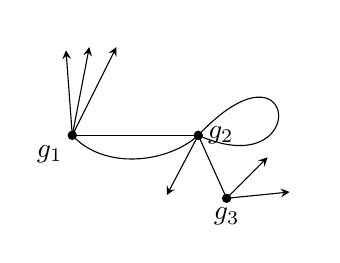
\begin{tikzpicture}[x=0.8cm,y=0.8cm,>=stealth]
\coordinate (s1) at (0,0);\coordinate (s2) at (2,0);\coordinate (s3) at (2.45,-1);
\draw (s1)--(s2);\draw (s1) .. controls (0.5,-0.55) and (1.5,-0.45) .. (s2);
\draw (s2) .. controls (3.6,1.7) and (3.8,-0.8) .. (s2);
\draw (s2)--(s3);
\draw[->] (s1)--(-0.1,1.35);\draw[->] (s1)--(0.27,1.4);\draw[->] (s1)--(0.7,1.4);
\draw[->] (s2)--(1.5,-0.95);\draw[->] (s3)--(3.1,-0.35);\draw[->] (s3)--(3.45,-0.9);
\fill (s1) circle (1.7pt);\fill (s2) circle (1.7pt);\fill (s3) circle (1.7pt);
\node[below left] at (s1) {$g_1$};\node[right] at (s2) {$g_2$};\node[below] at (s3) {$g_3$};
\end{tikzpicture}}

\margin{\deleted{\unsure{orientations}} \unsure{pondérés} \uline{\unsure{comme d'hab.}} \deleted{\unsure{MD}}}

Condition de stabilité MD :
\[
(4)\qquad \forall s\in S,\ \text{on a }2g_s+\widehat\nu_s\geq3\quad\text{i.e.}\quad
\left\{\begin{array}{l}
g_s=0\ \Rightarrow\ \widehat\nu_s\geq3\\
g_s=1\ \Rightarrow\ \widehat\nu_s\geq1
\end{array}\right.
\]
\margin{graphes \uline{stables} : qui satisfont la condition (4)}

i.e. $\widehat\nu_s$ est le nb d'arcs \deleted{qui} d'origine $s$ (\uline{ordre total} du sommet $s$) tandis que $\nu_s$ désignera le nb d'arcs ordinaires, donc
\[
(5)\qquad
\underset{\substack{\uline{\text{ordre total}}\\\text{de }s}}{\widehat\nu_s}
=
\underset{\substack{\uline{\text{ordre}}\\\deleted{\unsure{\text{total}}}\\\uline{\unsure{\text{réduit}}}\\\text{de }s}}{\nu_s}
+
\overset{\substack{\unsure{\operatorname{card}I}\ \text{si }I=\widehat{\vec A}^{\sigma}}}{
\underset{\substack{\uline{\text{ordre complémentaire}}\\\text{de }s\\\text{(correspondant}\\\text{aux ``pts marqués''}\\\text{sur une courbe alg.)}}}{\unsure{\vec\nu_s}}}
,\quad \uline{\text{``marqué''}}
\]
\deleted{$\unsure{\nu_s}=2\unsure{\nu'_s}\quad\unsure{\nu'_s}\ \unsure{\text{nb d'arêtes}}$}

\margin{Si le graphe est connexe, le couple $(g,\nu)$ est \unsure{appelé} son type numérique. Dans le cas général, on lui associe \unsure{l'invariant numérique}, \unsure{spécifié} par une application
\diagram{\begin{tikzcd}
\uline{I}\arrow[r]&\pi_0(G)\arrow[r,"g","\substack{\text{genre}\\\text{virtuel}\\\text{d'une}\\\text{composante}}"']&\mathbb N
\end{tikzcd}}}

On pose
\[
(6)\qquad \nu=\nu(G)\deleted{\unsure{\nu_G}}=\sum_s\unsure{\vec\nu_s}=\operatorname{card}(\vec A^{\sigma})\quad
(\uline{\text{ordre marqué}}\ \deleted{\unsure{\text{tot}}}\ \text{du graphe})
\]
\[
(7)\qquad c=c(G)=\deleted{\unsure{\nu}}\frac12\sum_s\nu_s
\qquad\text{nb des arêtes ordinaires : }\uline{\text{codim.}}\ \uline{\text{modulaire}}\ \text{du graphe}
\]
\[
(8)\qquad g=\sum_{s\in S}g_s+\underset{\substack{\unsure{\text{connexité}}\\\text{de }G}}{\underbrace{h^1(G)}}.
\quad\uline{\text{genre virtuel}}\ \text{du graphe}
\]
(correspond à $\dim H^1(X,\unsure{\mathcal O_X})$)
\scanpage{129}
\deleted{$\unsure{g_i}$}

\deleted{\unsure{(8)}} Si le graphe est MD, alors $(g,\nu)$ est admissible, et on pose
\[
(9)\qquad \unsure{\delta|d}(G)=\unsure{3}g-3+\nu
\qquad (\uline{\text{dimension}}\ \text{modulaire}\inserted{\uline{ambiante}})
\]
et on aura
\[
(10)\qquad d(G)+c(G)=\delta(G)
\]

\uline{Opérations} \inserted{\uline{et morphismes}.}
Soit $G,G'$ \deleted{deux} graphes MD, on appelle \uline{hom de générisation} \inserted{$u$} de $G$ dans $G'$ un couple d'applications
\diagram{\begin{tikzcd}[row sep=small]
S\arrow[r,"u_s"]&S'\\
\widehat{\vec A}\arrow[r,"u_a"]&\widehat{\vec A}'\amalg S'
\end{tikzcd}}
satisfaisant les conditions suivantes, où
\[
\vec B=u_a^{-1}(\widehat{\vec A}'),\qquad
\vec C=\widehat{\vec A}\setminus\unsure{B}=u_a^{-1}(S')
\]
a) $\vec B\supset I$ (ens des arcs libres), $\vec B$ stable par $\sigma$

b) L'application $\vec B\longrightarrow\widehat{\vec A}'$ induite par $u_a$ commute aux involutions et le couple $(u_s,u_a|\vec B)$ \unsure{commutent|commute} aux applications origine.
(Donc $u_a$ induit $I\longrightarrow I'$)

\margin{i.e. $(S,\vec B)$ \deleted{\unsure{a}} définit un sous-graphe de $(S,\widehat{\vec A},o,\sigma)$ contenant les arêtes libres de $G$; $(u_s,u_a|\vec B)$ définit un hom. de graphes.}

c) \deleted{$\unsure{a\in\vec C}$} si $c\in\vec C$, alors
\[
u_a(c)=\inserted{u_a(-c)=}u_s(\underbrace{o(c)}_{\text{origine}})
\]
(donc $u_a|C$ est connu quand on \unsure{connaît|connait} $u_s$)\deleted{\unsure{a}}. \unsure{donc}
[Donc \deleted{\unsure{de $u_s$ doit}} $u_s$ a même image sur deux \deleted{\unsure{les}} sommets $s,s'$ tels que $\exists c\in\vec C$, $s=o(c)$, $s'=o(-c)$ --- donc $u_s$ se factorise en
\diagram{\begin{tikzcd}
S\arrow[r]&S/R\arrow[r]&S'
\end{tikzcd}}
où $R$ est la relation d'équivalence dans $S$ engendrée par la relation précédente]

d) $S/R\longrightarrow S'$ induit par $u$ est une bijection,
$\vec B\longrightarrow\widehat{\vec A}'$ est une bijection

\margin{donc $S'$ et $\widehat{\vec A}'$ se récupèrent à partir de $\vec B\subset\widehat{\vec A}$ i.e. de $C$, à bijection can. près\ldots}

e) Pour tout $s'\in S'$, soit $S(s')=u_s^{-1}(\{s'\})$, $\unsure{\vec C(s')|\widehat{\vec A}(s')}=$ ens. des $\alpha\in\deleted{\unsure{\widehat A}}\vec C$ tels que
\deleted{$u_a(\alpha)=s'\ \text{ou}\ \unsure{u_a(\alpha)}$}
$o(\alpha)$ et $e(\alpha)\in S(s')$
(i.e. $u_a(\alpha)=s'$)
\deleted{ou $\alpha\in B$ et $\unsure{o'(u_a(\alpha))=e'(u_a(\alpha))=s'}$)}.
Soit \deleted{alors} $G_0(s')$ le sous-\deleted{\unsure{MD}}-graphe \inserted{pondéré} de $G$ défini par $S(s')$ et $\unsure{\widehat{\vec A}(s')}$, considérons son genre virtuel
\[
\uline{g}(G_0(s'))=\sum_{s\in S(s')}g_s+h^1(G_0(s'))
\]
\margin{\uline{NB} d) assure que $G(s')$ est connexe}
On a alors
\[
\uline{g}_{s'}=g(G_0(s'))
\]
\mspage{128}
\scanpage{130}
\uline{NB} Le \inserted{MD-}graphe \deleted{\unsure{par}} $G'$ se déduit, à isom. unique près, de $G$ et de $C\inserted{=\vec C/\sigma}\subset A=\underbrace{A(G)}_{\substack{\text{ens. des arêtes}\\\text{liées}}}$.
Soit $\unsure{G_{0C}^{c}}$ le sous-graphe de $G$ défini par
\[
\begin{array}{l}
S(G_{0C})=S\\
\vec A(G_{0C})=\vec C\quad(\text{image inv. de }C\text{ dans }\widehat{\vec A})
\end{array}
\]
pondéré par $\uline{g}:\unsure{S}=S(G_{0C})\longrightarrow\mathbb N$ provenant de $G$.

On pose
\[
\left\{\begin{array}{l}
S'=\pi_0(G_{0C})\\
\unsure{\widehat{\vec A}'|\widehat A'}=\widehat{\vec A}\setminus\vec C\ \deleted{=\unsure{B}}\\
o':\widehat{\vec A}'\longrightarrow S'\quad\text{composé}\\
\sigma'\ \text{induit par }\sigma\\
g_{s'}=\text{genre virtuel de la comp. connexe}\\
\hfill G_{0C,s'}\ \text{du graphe pondéré }G_{0C}
\end{array}\right.
\]
\margin{où $\vec C$ est l'image inverse}
\diagram{\begin{tikzcd}[column sep=small,row sep=small]
\unsure{\widehat{\vec A}'}\arrow[r,hook]&\widehat{\vec A}\arrow[r,"o"]&S=S(G_{0C})\arrow[r,"\text{can.}"]&S'\arrow[d,equal]\\
&&&\pi_0(G_{0C})
\end{tikzcd}}

\uline{NB} On aura $I\simeq I'$, $\pi_0(G)\xrightarrow{\sim}\pi_0(G')$ et les applications $\gamma:\pi_0(G)-\mathbb N$ et $\gamma':\pi_0(G')-\mathbb N$ (genre virtuel d'une composante) se correspondent.

\mspage{129}
\scanpage{131}
\mspage{130}

1) \deleted{Sectionnage}\inserted{Découpage} (d'arêtes) et recollage (de bouts d'arcs libres)
$\Longleftrightarrow$ normalisation partielle et recollage par identifications)

Si $G$ et $G'$ se correspondent, ($G'$ déduit de $G$ par découpage)
\[
M_G\simeq M_{G'},\qquad \widehat M_G\simeq\widehat M_{G'}\qquad
\mathcal X_{G'}\longrightarrow\mathcal X_G,\quad \widehat{\mathcal X}_{G'}-\widehat{\mathcal X}_G
\]
\uline{NB} On a $S=S'$ et $g_s=g'_s$, $\widehat\nu_s=\widehat\nu'_s$ --- mais \deleted{$\unsure{\nu}$} $\nu_s,\vec\nu_s$ \uline{changent}.

Cette opération sert surtout pour exprimer \inserted{\unsure{un|ou}} $M_G$ -- $\widehat M_G$ comme un produit $\prod_{s\in S}M_{g_s,\unsure{\widehat{\vec A}_s}}$ resp $\prod_s\widehat M_{g_s,\widehat A_s}$.

2) Hom. ordinaire de \inserted{MD-}graphes \deleted{pondérés} (hom de graphes, compatible avec pondération) $\unsure{G'|G}\xrightarrow{u}\unsure{G|G'}$ (\unsure{carré|avec}
\diagram{\begin{tikzcd}
S\arrow[r]\arrow[dr,"\uline{g}"']&S'\arrow[d,"g'"]\\
&\mathbb N
\end{tikzcd}}
commutatif). On a alors
\[
M_G\longrightarrow M_{G'},\qquad
\deleted{\widehat M_G\longrightarrow\widehat M_{G'}}
\]
\[
\mathcal X_G\mathbin{\times}_{M_{G'}}\unsure{M_{G'}|M_G}\longrightarrow\mathcal X_G,\qquad
\deleted{\widehat{\mathcal X}_G\mathbin{\times}_{\widehat M_{G'}}\widehat M_G\longrightarrow\widehat{\mathcal X}_G}
\]
\margin{ne passe pas aux compactifiés}
(auquel d'ailleurs $\unsure{M_{G'}\longrightarrow M_G}$ se réduit)

\margin{Mais il faut supposer que $\forall s'\in S'$, l'application induite $\widehat{\vec A}'_{s'}\longrightarrow\widehat{\vec A}_s$ ($s=u(s')$) soit injective --- On dira que $u$ est une \uline{immersion}}

Cas particuliers intéressants : les hom de transition \deleted{\unsure{fonctorialité}} entre les $M_{g\nu}^{!}$ (qui déjà ne passent pas aux compactifiés !)

Hom d'induction de MD-graphes $G',G$, $u:G'-G$
\diagram{\begin{tikzcd}[column sep=large]
S'\arrow[r,"u_0"]&S
\end{tikzcd}}
\diagram{\begin{tikzcd}[column sep=large]
\widehat{\vec A}'=I'\amalg\vec A'\arrow[r,"u_1"]&\widehat{\vec A}=I\amalg\vec A
\end{tikzcd}}

satisfaisant

a) compatibilité aux applications \uline{origine}
\diagram{\begin{tikzcd}
\widehat{\vec A}'\arrow[r,"u_1"]\arrow[d,"o'"']&\widehat{\vec A}\arrow[d,"o"]\\
S'\arrow[r,"u_0"']&S
\end{tikzcd}}
comm.

(mais pas compatible aux applications extrémité, ni aux $\sigma$\inserted{$\sigma'$})

b) $\overbrace{u_1^{-1}(I)}^{I'_0}\subset I'$ i.e. $u_1^{-1}(\vec A)\supset\vec A'$ i.e. $u_1(\vec A')\subset\vec A$
et on veut que sur $\vec A'$, $u_1$ commute à $\sigma,\sigma'$.

\deleted{c) \unsure{Rq} $I'_1=I'\setminus I'_0=I'\cap u_1^{-1}(\vec A)$, i.e. on veut que $u_1(I'_1)\subset\vec A$ soit stable par $\sigma$, et $u_1|I'_1$ injectif}

\inserted{c) $u_1:\widehat{\vec A}'_{s'}\longrightarrow\widehat{\vec A}_s$ ($s=u_0(s')$) est \uline{injectif}}
\scanpage{132}
U N I V E R S I T E\\
DES SCIENCES ET TECHNIQUES\\
DU LANGUEDOC\\
\texttt{------------}

Montpellier, le 25 Novembre 1981

Service de la Scolarité\\
MA / GJ\\
Diffusion : Liste A\\
N° : 6455

AVIS DE SOUTENANCE D'UNE THESE DE DOCTORAT DE 3ème CYCLE

CHIMIE ORGANIQUE PHYSIQUE\\
\texttt{-------------------------}

\uline{Nom et prénom du candidat} : LORENTE Philippe

\uline{Titre de la thèse} : HYDROLYSE D'ORTHOESTERS CYCLIQUES AROMATIQUES\\
Compétition entre effet stéréoélectronique et effet de groupe partant.

\uline{Date, heure et lieu de soutenance prévus} :\\
11 DECEMBRE 1981 à 16 Heures\\
Salle de Cours n° 2 - USTL

\uline{Nom du Directeur de thèse} :\\
Monsieur le Professeur G. LAMATY

\uline{Désignation du laboratoire où la thèse est préparée} :\\
Laboratoire de Chimie organique physique.

\uline{Résumé de la thèse} :

Quatre orthoesters cycliques aromatiques dérivés de la dihydro-3,4 coumarine substituée sur le noyau benzénique ont été synthétisés ; la réaction d'hydro-\\
lyse de ces composés a été étudiée dans le but d'opposer un effet de groupe partant à l'effet stéréoélectronique qui se manifeste dans ce type de réaction.Une évaluation de l'énergie due à l'effet stéréoélectronique pouvait résulter de l'étude de cette compé-\\
tition.

Deux hypothèses ont été formulées pour rendre compte des résultats expérimentaux ; l'une d'entre elle conduit à une estimation de l'énergie stéréoélectro-\\
nique.

\uline{Durée approximative des recherches ayant abouti à la thèse} : 2 ans

\uline{Composition du jury proposé} :\\
MM. : LAMATY Gérard\\
GENESTE Patrick\\
MOREAU Claude\\
VIALLEFONT Philippe

P. le Secrétaire Général,\\
l'Attachée d'Administration Universitaire,

\figure{
\begin{tikzpicture}[x=0.8cm,y=0.8cm,line width=0.6pt]
\draw (0.48,-0.6) .. controls (0.44,-0.04) and (0.55,0.9) .. (0.56,1.12)
 .. controls (0.45,1.3) and (0.45,0.85) .. (0.51,0.61)
 .. controls (0.26,0.98) and (0.32,0.58) .. (0.57,0.64)
 .. controls (0.77,0.72) and (0.8,0.65) .. (0.93,0.64);
\draw (0.52,0.58) .. controls (-0.09,0.22) and (-0.04,0.02) .. (0.42,0.1)
 .. controls (0.65,0.14) and (0.91,0.21) .. (0.9,0.22)
 -- (0.64,0.16) .. controls (1.11,0.11) and (1.87,0.13) .. (2.07,0.2)
 .. controls (2.22,0.24) and (2.24,0.53) .. (2.16,0.68)
 .. controls (2.05,0.79) and (2.14,0.29) .. (2.17,0.01);
\draw (2.17,0.2) -- (2.17,-0.02);
\draw (3.02,-0.03) .. controls (2.8,-0.12) and (0.37,-0.11) .. (0.26,-0.24)
 .. controls (0.15,-0.33) and (0.5,-0.31) .. (0.55,-0.3);
\draw (-0.02,0.17)--(-0.08,0.23);
\end{tikzpicture}}
A. GENTIL

\mspage{131}
\scanpage{133}
\unsure{d)} On a commutativité dans
\diagram{\begin{tikzcd}
S'\arrow[rr,"u_0"]\arrow[dr,"\uline{g'}"']&&S\arrow[dl,"\uline{g}"]\\
&\mathbb N&
\end{tikzcd}}.

Soit $X$ une courbe de type $G$, \inserted{sur un corps $k$}, on normalise
\diagram{\begin{tikzcd}[column sep=large]
\widetilde X=\coprod_{s\in S}\widetilde X_s&\widehat{\vec A}_k=\coprod_s(\widehat{\vec A}_s)_k\arrow[l]
\end{tikzcd}}
\margin{$X$ déduit de $\widetilde X$ par identification à l'aide de $\sigma$}

on \deleted{\unsure{va}} en déduira une courbe $X'$ de type $G'$, posons
\diagram{\begin{tikzcd}[column sep=small,row sep=large]
\widetilde X'=\coprod_{s'\in S'}\underbrace{\widetilde X'_{s'}}_{\substack{=\mathrm{déf}\\\widetilde X_{u_0(s')}}}\arrow[rr]&{}\arrow[dr,dash,bend right=30,"\text{défini via}"']&\widehat{\vec A}'_k=\coprod_{s'\in S'}(\widehat{\vec A}'_{s'})_k\\
&& (\widehat{\vec A}'_{s'})_k\lhook\joinrel\xrightarrow{\mathrm{inj}}(\unsure{\widehat{\vec A}_s|\widehat{\widehat{\vec A}}_s})_k\hookrightarrow\widetilde X_s=\widetilde X'_{s'}
\end{tikzcd}}
et on construit une $X'$ par identification à partir de $\widetilde X'$ via $\sigma'$, agissant \inserted{librement}, sur $\vec A'_k$. On a évidemment
\[
\overset{\deleted{\unsure{\sim}}}{X'}\longrightarrow\overset{\deleted{\unsure{\sim}}}{X}
\qquad\uline{\text{morphisme fini net}}
\]
appliquant $I'$ dans $I\amalg\operatorname{Sing}X$, et qui sur les \deleted{normalisées} comp. \unsure{irrd.|irred.} \deleted{\unsure{donne des isom.}}\inserted{des normalisées donne un iso}

Inversement, si on a un tel morphisme

\noindent - - - -

\vfill
\mspage{132}
\scanpage{134}
U N I V E R S I T E\\
DES SCIENCES ET TECHNIQUES\\
DU LANGUEDOC\\
\texttt{------------}

Montpellier, le 25 Novembre 1981

Service de la Scolarité\\
MA / GJ\\
Diffusion : Liste A\\
N° 6443

AVIS DE SOUTENANCE D'UNE THESE DE DOCTORAT DE SPECIALITE

MATHEMATIQUES APPLIQUEES\\
\texttt{------------------------}

\uline{Nom et prénom du candidat} : ROS Marius

\uline{Titre de la thèse} : Sur quelques questions de cinématique et de statique des surfaces.

\uline{Date, heure et lieu de soutenance prévus} :\\
10 DECEMBRE 1981 à 10 Heures\\
Salle 431 - Bâtiment des Mathématiques - USTL

\uline{Nom du Directeur de thèse} : Monsieur le Professeur MOREAU

\uline{Désignation du laboratoire où la thèse est préparée} : Mathématiques

\uline{Résumé de la thèse} :

Une membrane étant représentée par une surface différentiable, on étudie les conditions pour qu'un champ tensoriel symétrique soit le champ tensoriel des vitesses de déformation. Localement, tout champ tensoriel symétrique suffisamment différentiable peut être considéré comme un champ tensoriel des vitesses de déformation si la surface est localement, de type hyperbolique, elliptique ou parabolique ; cela n'est plus vrai dans le cas localement plan. Globalement, des théorèmes d'unicité pour le champ vectoriel des vitesses correspondant sont obtenus dans le cas des surfaces simplement connexes de type hyperbolique ou elliptique. Ceci entraîne la rigidité de certaines membranes en mouvement isométrique dont le bord est rigide. Un résultat corré-\\
latif est que, pour une membrane de même forme, en équilibre en l'absence de forces extérieures, le champ tensoriel des contraintes est nul.

\uline{Durée approximative des recherches ayant abouti à la thèse} : 4 ans

\uline{Composition du jury proposé} :\\
MM. MOREAU J.-J.\\
JOUANNA P.\\
MAISONNEUVE O.

P. le Secrétaire Général,\\
L'Attachée d'Administration Universitaire,

\figure{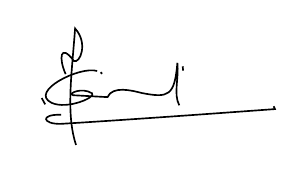
\begin{tikzpicture}[x=0.004cm,y=-0.004cm,line width=0.6pt]
\draw (678,430) .. controls (645,330) and (665,200) .. (675,60)
 .. controls (718,107) and (690,173) .. (671,163)
 .. controls (628,105) and (622,154) .. (645,205);
\draw (745,195) .. controls (691,178) and (527,260) .. (600,296)
 .. controls (650,319) and (743,278) .. (729,266)
 .. controls (698,245) and (648,267) .. (669,272)
 -- (778,278) .. controls (794,241) and (856,257) .. (887,265)
 .. controls (971,281) and (991,276) .. (1000,169)
 .. controls (1005,219) and (987,269) .. (1006,304);
\draw (1017,180)--(1018,194);
\draw (756,199)--(761,204);
\draw (569,281)--(580,301);
\draw (631,334) .. controls (562,332) and (572,364) .. (629,363)
 .. controls (842,350) and (1104,331) .. (1310,316)--(1306,307);
\end{tikzpicture}}
A. GENTIL

\mspage{133}
